 \documentclass[journal]{IEEEtran}
\IEEEoverridecommandlockouts
\usepackage{cite}
\usepackage[cmex10]{amsmath}
\usepackage{graphicx}
\usepackage{graphics}
 \usepackage{epstopdf}
\usepackage{subfigure}
\usepackage{epsfig}
\usepackage{algorithmic}
\usepackage[linesnumbered,ruled,slide]{algorithm2e}
\usepackage{amsfonts}
\usepackage{float}
\usepackage{enumerate}
\usepackage{verbatim}
\usepackage{caption3}
\usepackage{bm} %%公式加粗
\usepackage[justification=centering]{caption}


\begin{document}

\title{1-Bit Compressive Sensing  Based Acoustic Source Localization  in  Dual-Microphone Array}

%
\author{\IEEEauthorblockN{Xin Zhou, Naigao Jin, Mingyi Yang, Xinyang Liu, Lei Wang\thanks{Naigao Jin is the corresponding author.}  }\\
\IEEEauthorblockA{School of Software, Dalian University of Technology, China\\
Email: ngjin@dlut.edu.cn, lei.wang@dlut.edu.cn, zhouxin964@gmail.com}
}

% make the title area
\maketitle

\thispagestyle{plain}
\pagestyle{plain}

\begin{abstract}
%\boldmath
Acoustic source localization in sensor network is a challenging task because of severe constraints on cost, energy, and effective range of sensor devices.
To overcome these limitations in existing solutions, this paper formally describes, designs, implements, and evaluates a 1-bit compressive sensing method to acoustic source localization, i.e., CS-ASL, in distributed smartphone networks.
We  collect the 1-bit binary left/right data  by estimating the sign of TDOA between the synchronized dual microphones. 
The key idea behind CS-ASL is to turn the localization  into sparse recovery problem of 1-bit  compressive sensing. 
The proposed design is evaluated through extensive simulations and physical experiments in an indoor test-bed with 30 smartphone nodes. Evaluation results show that CS-ASL  can effectively locate the acoustic source with good robustness.



\end{abstract}

\begin{IEEEkeywords}
Compressive Sensing, Acoustic Source Localization,  Dual-Microphone Array, Sparse Recovery
\end{IEEEkeywords}



\IEEEpeerreviewmaketitle
\input{Introduction}
\section{System Model}


In our work, we use the dual-microphone smartphones to collect the acoustic signals.
The binary left/right data is achieved by leveraging the sign of time-difference-of-arrival (TDOA) of the sound at the two phone microphones. Here we bring in the perpendicular bisector of the double microphones, according to the acoustical signal received by smartphone, judging the acoustical source in the left or in the right of the perpendicular bisector. We set that in the clockwise direction if acoustic source in the left we describe the measure data as 0, otherwise if in the right we define it as 1. Compared with traditional method, we use the 1-bit data instead of the concrete TDOA values, which is robust to measurement error.

  \begin{figure}[!htb]
	\centering
	\setlength{\abovecaptionskip}{-15pt}
	\vspace{-3mm}  
	%\setlength{\belowcaptionskip}{-5pt}
	\includegraphics[width=6cm,height=4.0cm]{image/b.pdf} 
	\vspace{3mm}
	\caption{System model}
	\label{fig2}
	\vspace{-5mm}
\end{figure}

As is shown in Fig.1, every lines can divide the space into two parts, when the lines increase to $n$, the space can be divided into $\frac{n^2+n+2}{2}$ parts at best. As long as the number of the smartphones is adequate,  the area of the subdomain is adequately accurate to represent the source location. 
Our target is searching for the points in the target subdomain using the 1-bit measure datas. We make the space gridding with large scale, transform the area into a large number of points.
The points inside the target subdomain are sparse compared with the whole points, satisfy the character of compressive sampling.
%As long as we compress the whole points by 1-bit measure data constantly, finally lead to the points in target subdomain. 
We regard the points in the target subdomain as the final target points, utilizing the average of these points to determine the location of the acoustical source.

Here, we talk about our 1-bit CS framework, considering the scene in the 2D space with $n$ points and $m$ smartphones, $n$ is large that can present the whole localization area, all points are ${S} = \{ {poin{t_1}}, \cdots ,{poin{t_i}}, \cdots ,{poin{t_n}}\}$, where any node ${poin{t_i}}$ has its location coordinate denoted as $[{x_i},{y_i}]$. The acoustic event occurs at ${O_s}{\rm{ = [}}{x_s},{y_s}]$. As for the $m$ smartphones, we utilize the midperpendicular of the two microphones, transform them to $m$ lines, where the ${lin{e_i}}$ is described as ${a_i}x+{b_i}y+{c_i}=0$, stipulate $a_i$ is a positive number all the time.  And the data we measure from every smartphone can be defined as
\begin{equation}\label{eq:eps}
D_{i}=
\left\{\begin{matrix}
1 ~~ $if$~~    {a_i}{x_s}+{b_i}{y_s}+{c_i}\geq0,\\
0 ~~ $if$~~   {a_i}{x_s}+{b_i}{y_s}+{c_i}<0,
\end{matrix}\right.
\end{equation}
where $1\leq i \leq m$, our target is to find few points among all the $n$ points when substituting it to the $m$ lines that most approaches to the $D$. Here, we confirm the average of the points to be the real source acoustic location.

We describe the localization model in the matrix form. Coefficient matrix $A$ is denoted as
\begin{equation}\label{eq:eps}
A=\begin{bmatrix}
&a_1  &b_1 &c_1 \\
&a_2  &b_2 &c_2\\
&.&.&. \\
&.&.&. \\
&.&.&. \\
&a_m  &b_m  &c_m
\end{bmatrix}
\end{equation}which indicates the $m$ lines and the point matrix is expressed as
\begin{equation}\label{eq:eps}
S=\begin{bmatrix}
&x_1 &x_2 &. &. &. &x_n \\
&y_2 &y_2 &. &. &. &y_n\\
&1  &1 &. &. &. &1
\end{bmatrix}
\end{equation} 


We represent the unknown target positions on a location grid as a sparse $n\times$1 vector $X$, calculating $X$ to determine whether ${poin{t_i}}$ in the target subdomain, for the points in target area, in matrix $X$ we set their index location as 1, as for other points we give their index value 0. 
To sum up, we conclude our localization model to a formula
\begin{equation}\label{eq:eps}
Sign(ASX)=D
\end{equation}
Provided we solve the matrix $X$, then leading to the points in target subdomain, utilize their average value to represent the location of the acoustic source.  After all concepts are put forward, we introduce the design of our localization method.



\section{DESIGN}

In this section,  we introduce the design of CS-ASL system. The key idea behind CS-ASL is to turn the localization into sparse recovery problem of 1-bit compressive sensing.  
Firstly, we introduce a CS-ASL-BF method with brute force. Then we describe a CS-ASL-GD method with gradient descent. After the two methods are proposed, we do further local refinement to improve the accuracy of the localization.

\subsection{CS-ASL-BF with brute force}
CS-ASL-BF is based on the idea of brute force searching. Grid meshing leading to a large number of points, we checkout them one by one with brute force searching, consider whether the point we are searching for is the one in target subdomain. Every point can reach an assumed measure vector by the relative location to $m$ lines, we believe the point with its assumed measure vector most approach to matrix $D$ is what we search for. In our CS framework, for the ${poin{t_i}}$ searching in matrix $X$ we set its index location as $1$ and other location as $0$, leading to an error matrix

\begin{equation}\label{eq:eps}
error_i=sign(ASX_i)-D
\end{equation}where $1\leq i \leq n$, every point of $n$ maps an error matrix, in that matrix defines none-zero numbers $\bm{nnz{_i}}$ as the cost function of that point. Finally the points with the minimum of cost function are in the target subdomain and their average value is the location we ultimately determine.



\subsection{CS-ASL-GD with gradient descent}
CS-ASL-BF performs extremely well in practical test. It can even obtain a high precision location when bit-flipping or other measure errors occur.
However, when we get an accurate location, meanwhile the huge number of the point searchings lead to high time complexity, which may slow down our system. To strengthen our method, we put forward a CS-ASL-GD method using gradient descent to confirm the real source acoustic point instead of searching for one point by one point.

We can turn the location problems to solve the linear equation with one unknown. One classical method in signal processing fields is bringing in gradient, searching for the points with maximum probability in every iteration process by gradient descent, in result, determine the real source acoustic point in the final time. CS-ASL-GD method is based on it.

Here our estimated matrix $X$ represents the probability of the $n$ points in target subdomain. Each iteration, we calculate the gradient at first, then update the probability of the $n$ points according to the step-size that gradient decreases by. 
\begin{equation}\label{eq:eps}
\varDelta=sign(ASX)-D
 \end{equation}Eq.6 means the increment of the functional value.
 \begin{equation}\label{eq:eps}
\bigtriangledown=sign((AS)'*\varDelta)
 \end{equation}Eq.7 gets the gradient $\bigtriangledown$ in Eq.4, aiming to get a solution to vector $X$. 
 \begin{equation}\label{eq:eps}
X=X-\mu *\bigtriangledown
 \end{equation}Eq.8 figures out a new probability of the $n$ points. $\mu$ present the gradient descent step, in traditional gradient descent process choosing an appropriate step-size $u$ is essential. If that value is large, we cannot obtain a more accurate probability. Otherwise if the value is too small, the change of the probability will be unapparent. One of the advantages of our 1-bit CS framework is that we introduce the sign function,  utilizing the 1-bit 0/1 information instead of concrete measure data, not only make iteration rapidly convergence but provides adequate slacks to construct gradient descent without an extremely accurate step-size. We choose the points with the maximum probability in vector $X$, confirming other points outsides the target area. Every iteration process excludes a large number of unnecessary points, which can rapid convergence to the area with acoustic source.
 \begin{equation}\label{eq:eps}
\hat{X_{i}}=
\left\{\begin{matrix}
1 ~~ $if$~~    X_i=max(X),\\
0 ~~ $if$~~   X_i \neq max(X),
\end{matrix}\right.
 \end{equation}where $1\leq i \leq n$, Eq.9 introduces a vector $\hat{X}$,  the points with maximum probability are all set 1, consider they  has the same probability to exist in target subdomain in this iteration,  no more determine the source location with other points. Then we use Eq.10 to make normalization processing, guarantee vector $X$ record the probabilities of the whole points, as input to next interation.
 \begin{equation}\label{eq:eps}
 X=\hat{X}/\sum\limits_{i=1}^n\hat{X_{i}}
 \end{equation}
 
 Several iterations later,  the probability of few points in vector $X$ keeps a large and stable value. Eventually, we regard the index points with a nonzero  value in  vector $X$ as the target points in our localization area.
 
 However, in real situations the kinds of error especially bit flipping seriously affect the performance of the system. Since what the gradient descent method search for is optimal points in one part, when bit-flipping occurs, the points we obtain often include several points outside the target sub-region without any handling. Here we  make the points gathering from gradient decease method as suspicious points, then adapt the CS-ASL-BF method to suspicious points for further searching, believe the points with nonzero value in matrix $X$ as the final points in real localization area.
 


\subsection{CS-ASL-LR with local refinement}
In our 1-bit CS framework, we utilize the sampling points in target subdomain to present the acoustic source. CS-ASL-BF  with brute force can find the whole points in target subdomain even occurs bit-filpping, as a result may slow down the system efficiency. CS-ASL-GD with bit fipping tolerance brings in gradient descent, although can get results fast, only determine several points in the target area not the whole points, leading to localization error in certain degree, which makes its accuracy inferior to CS-ASL-BF in high error conditions especially bit-flipping. Here we regard the CS-ASL-BF as the best accuracy  standard, making more efforts to make the accuracy of the CS-ASL more  approach to CS-ASL-BF with high efficiency. Aiming at above question, we have once considered finding the bit flipping nodes in the process of iterations, recover them and localize again by CS-ASL-GD method. However,  CS-ASL-GD has determine a more precise location, repeat work only make the system more complicated. Owing to the area of the target subdomain is adequate small, only make further amelioration searching by CS-ASL-BF method for the points neighbor to the location determined by CS-ASL-GD method can overcome this limit without raising much complexity. Results collect more points belong to the target subdomain leading to a more accurate localization.
%Traditional localization usually use the concrete measurement values to get an accurate location. However, the errors in the measurement seriously affect the performance. In this paper, we utilize the 1-bit information about the acoustic source on the left or on the right of the midperpendicular of the double microphones phones instead of the concrete measurement values, which leads to enough slack for localization in real error situations. As long as the number of the sensors is sufficient, as the area of the subdomain divided by  midperpendicular decreases, finally determine the points in final subdomain as the target. Basic 1-bit CS performs better even in high error environment, it can find the whole points in target subdomain, however every point has to calculate one time which tremendously slow down the efficiency. Although the points obtaining from the advanced 1-bit CS is inside the target subdomain, what it finds is some not all points, leading its behavior inferior to basic 1-bit CS especially in high error conditions. We make further amelioration searching for the points neighbor to the points that we have found in target subdomain by basic 1-bit CS. Results collect more points belong to the target subdomain leading to a more accurate localization.
  
 
   

%For the sake of presentation, until now we have described HPI-SBL in an ideal case where a complete and perfect node sequence can be obtained.
%In this section, we describe how to make HPI-SBL work well under more realistic conditions.
%
%%Basic HPI-SBL can find a solution to this feasibility program only if there is a region satisfying all the constraints.
%In the practical application, if two nodes are very close to each other along the direction of event propagation, they would detect the event almost simultaneously.
%In this case, the node order in the sequence may occur flip.
%%For instance, the true sequence is $NodeSeq ( \cdots ,i,j, \cdots )$, but the detected sequence is $NodeSeq ( \cdots ,j,i, \cdots )$.
%Basic HPI-SBL might fail to find a feasible solution that satisfies all the constraints when sequence flip occurs.
%For example, as shown in Fig. 2, the right middle region identifies by the node sequence $NodeSeq (D B C A)$.
%Once the order of node A and C occurs flip in $NodeSeq (D B C A)$, the region corresponding to $NodeSeq (D B A C)$ will not exist, basic HPI-SBL can not give the accurate estimation.
%In this section, we propose a robust solution to address the problem of sequence flip, called probabilistic HPI-SBL.
%
% Considering the uncertainty of the measurement with the node sequence $NodeSeq( \cdots ,i,j, \cdots )$, the probability of ${d_i} < {d_j}$ can be described as
% \begin{equation}\label{eq1}
% ASW=D
% %p({d_i} < {d_j})>\alpha
% \end{equation}
%Eq.\ref{eq1} means that the probability of the acoustic source in the left side of the the half-plane $H_{ij}$ is $\alpha$, and the right side is $1-\alpha$.
%After dividing the localization space into some discrete grids, the weight of the grid point in the left side of the the half-plane $H_{ij}$ is $\alpha$, and the weight of the grid point in the right side of the the half-plane $H_{ij}$ is $1-\alpha$.
%
%Besides these key constraints mentioned in Basic HPI-SBL, we can also have some relaxed constraints during the construction of the half plane.
%For example, given $NodeSeq (A C B D)$, we can get three key constraints $SA<SC$, $SC<SB$ and $SB<SD$ from the two adjacent nodes;
%and some relaxed constraints $SA<SB$, $SA<SD$ and $SC<SD$ from the two nonadjacent nodes in the node sequence.
%Given the node sequences with $N$ nodes, we can use all  $N(N - 1)/2$  constraints to further improve the localization robustness.
%By processing  $N(N - 1)/2$ half-planes, we can compute the cumulative weight $w$ of each discrete grid point $\bm{x}$
%
%\begin{equation}\label{eq2}
%w(\bm{x})=\sum\limits_{k=1} ^{N-1}\alpha(k).
%\end{equation}
%The region with the highest probability is the final region of the acoustic source
%\begin{equation}\label{eq3}
%\hat{\bm{X_s}}=arg \max_{\bm{x} \in R}w(\bm{x}).
%\end{equation}
%The centroid of the final region is the estimated location of the acoustic source.
%
%To summarize, the probabilistic HPI-SBL is presented in Algorithm 1.
%The input are the node sequences and anchor locations; the output is the location of the acoustic source.
%Step 1 sets the the initial weight of each discrete grid point.
%Step 2 uses the node sequence to get multiple half-planes, then computes the cumulative weight.
%Step 3 adopts the center of the final intersection region as the location of acoustic source.
%
%\begin{algorithm}
%\caption{Probabilistic HPI-SBL}
%\KwIn { The location of $N$ smartphones \\
%\hspace{0.41in} The node sequence of the acoustic source for\\
%\hspace{0.41in} $N$ smartphones
%}
%\KwOut {Location of the acoustic source}
%
%\textbf{Step 1:} Setting the weight of each grid point  $w(k) \leftarrow 0$;
%
%\textbf{Step 2:} Computing the cumulative weight by processing node sequence: \\
%\hspace{0.0in} Contructing half planes by processing node sequence;\\
%\For{$i \leftarrow 1$ \textbf{to} $N-1$}
%{
%\For{$j \leftarrow i+1$ \textbf{to} $N$}
%{
%Contructing half plane $H_{ij}$\\
%Updating Weight $w(k)$ for each grid point;\\
%}
%}
%\textbf{Step 3:} The center of region with the highest probability is the location of acoustic source.
%\end{algorithm}
%
%\subsection{Bit Flips}
%
%
%\iffalse
% \subsection{Complexity Analysis}
% This section provides the complexity analysis for the proposed
% LPSBL design. It needs to be emphasized that
% LPSBL itself adopts an asymmetric design in which sensor
% nodes need only to detect and report the events. Therefore,
% we only analyze the computational cost on the node sequence
% processing side, where resources are plentiful.
%
% SBL: Calculating the Spearman’s coefficient and Kendall’s Tau
% between two sequences are $O(N)$ and $O(N^2)$ operations,
% respectively. Since the location sequence table is of size
% $O(N^4)$, searching through it takes $O(N^5)$ and $O(N^6)$ operations,
% respectively~\cite{yedavalli2008sequence}.
%
% RSBL: Discrete space grid  M
%\fi



%\input{Discussion}
\section{EVALUATION }
\label{section:results}

\subsection{Simulation}
In order to verify our methods, demonstrating their behaviors in different conditions, we do a great deal of Monte Carlo simulator experiments randomly that design and implement the 1-bit CS method including CS-ASL-BF, CS-ASL-GD and CS-ASL-LR using MATLAB.
In our experiments, we simulate a 10m$\times$10m area with some smartphones as sensors deployed randomly and choose a point as acoustic source. Considering the uncertain conditions in real localization environment, we add different kinds of error including node location error, node angle error and the number of bit-flipping nodes aiming to show their good performances in different situations. We set the step of gradient descent $\mu$ as 0.5. Table 1 shows the major default parameter configurations in our simulations. Results are demonstrated in the followings.

%\iffalse
\begin{table} \normalsize
\caption {\textbf{Default configuration parameter}} %title of the table
\centering % centering table
    \begin{tabular}{|c|c|}
        \hline
\textbf{Parameter} & \textbf{Description} \\
 \hline
Field Area & 10m $\times$10m \\
\hline
Number of Anchors & 30 (Default) \\
 \hline
Node Location Error 	 & 0.2m (Default) \\
\hline
Node Angle Error & 5$^{\circ} $(Default) \\
\hline
Number of Bit-Flipping & 3 (Default) \\
 \hline
Random-Seed Loop	 & 1000 times  \\
% \hline
%Error Statistics	 &  RMSE \\
        \hline
    \end{tabular}
\end{table}
%\fi

\textbf{1) Impact of the number of anchors:}
 Here we choose the the number of anchor nodes from 10 to 40 in steps of 3, other parameter set the defaut values.
The results in Fig. \ref{Fig3:3-1} show that, with more node numbers, the whole area is divided into more multiple parts, and the subdomain we finally determine is more approach to the real acoustic source.
CS-ASL-BF is better for brute force searching for all points, but degrade the system efficiency. We utilize its localization accuracy as the best bound, compared with other two method to demonstrate  their performance. CS-ASL-LR enhances system efficiency in condition of localization accuracy guaranteed.
\iffalse 
 \begin{figure}[htb]
            \setlength{\abovecaptionskip}{0pt}
           % \centering
			 \vspace{-15mm}
           		 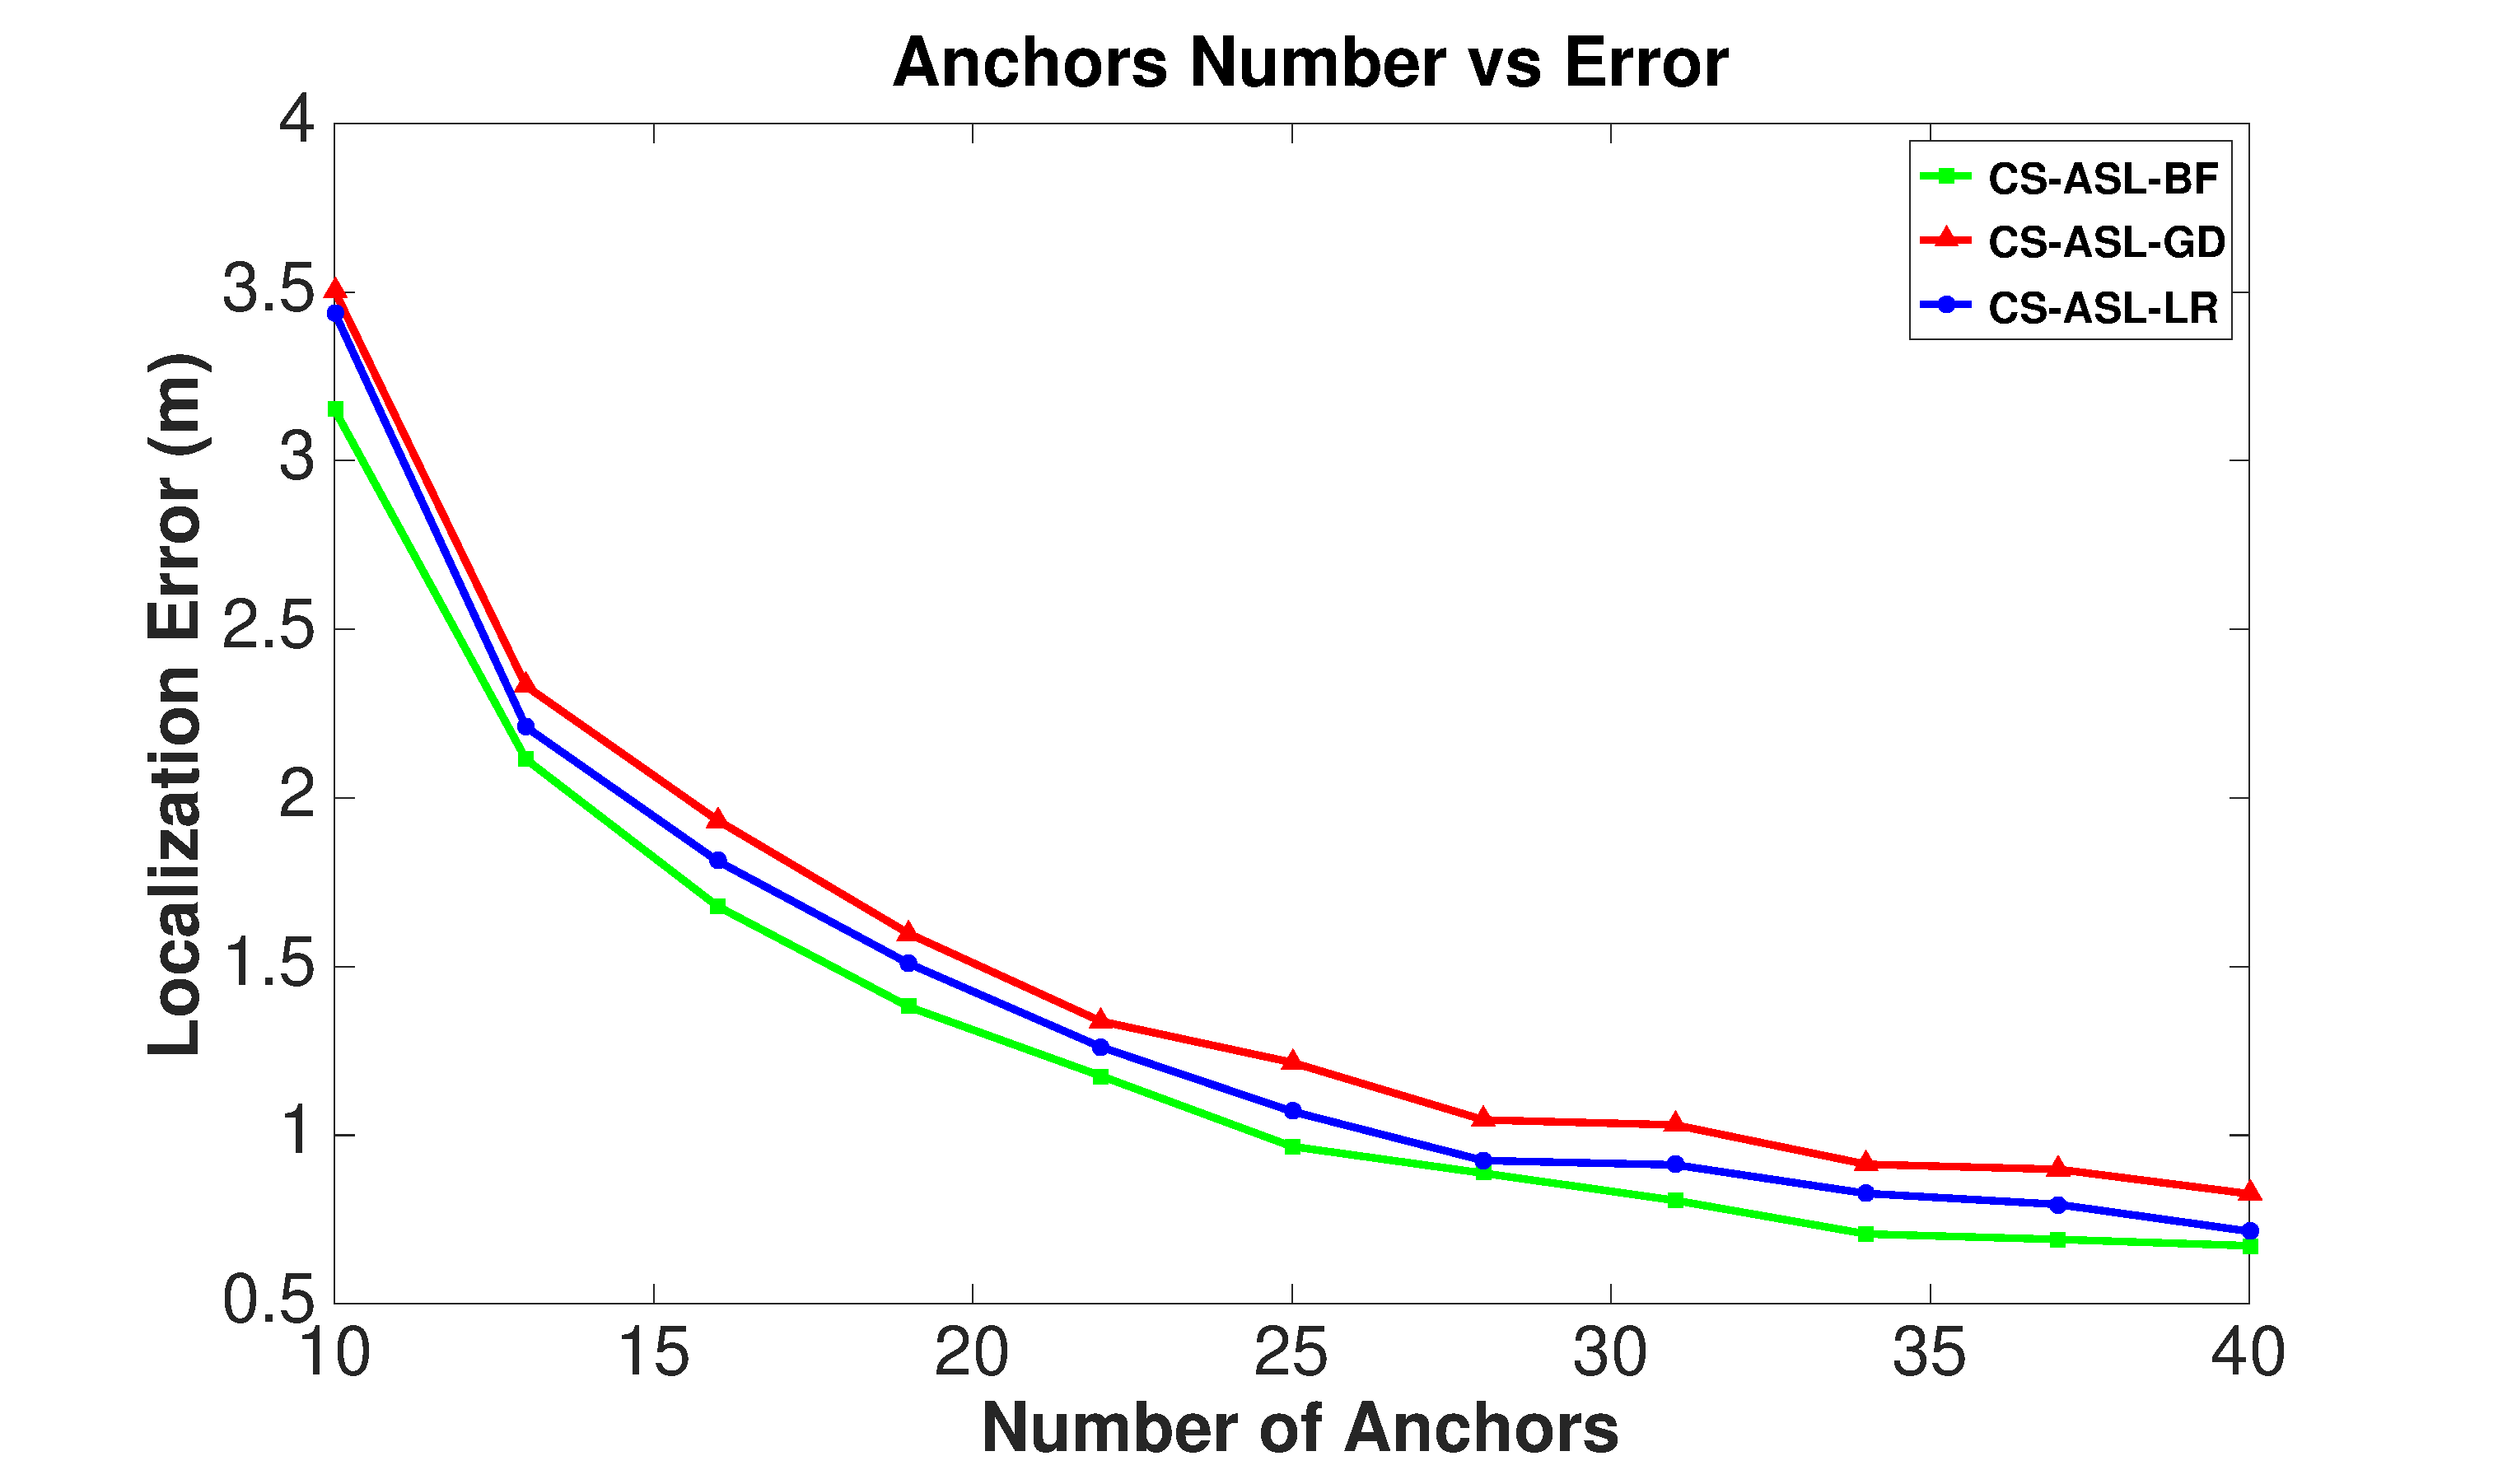
\includegraphics[height=5.0cm,width=7.0cm]{image/nodenumber.eps}
            \vspace{15mm}
            \caption{Localization Error vs. Number of Anchors}
             \vspace{-7mm}
             \label{fig4}
        \end{figure}
\fi
		
\textbf{2) Impact of the node location error:}
In this experiment we choose the location error from 0 to 0.5m in steps of 0.05m, other parameters remain the default. With the raisement of the node location error, Fig. \ref{Fig3:3-2} shows that the localization error increases slowly, even the error add to 0.5m our methods still have a good performance. 

\iffalse
  \begin{figure}[htb]
          %  \centering
		   \vspace{-25mm}
			 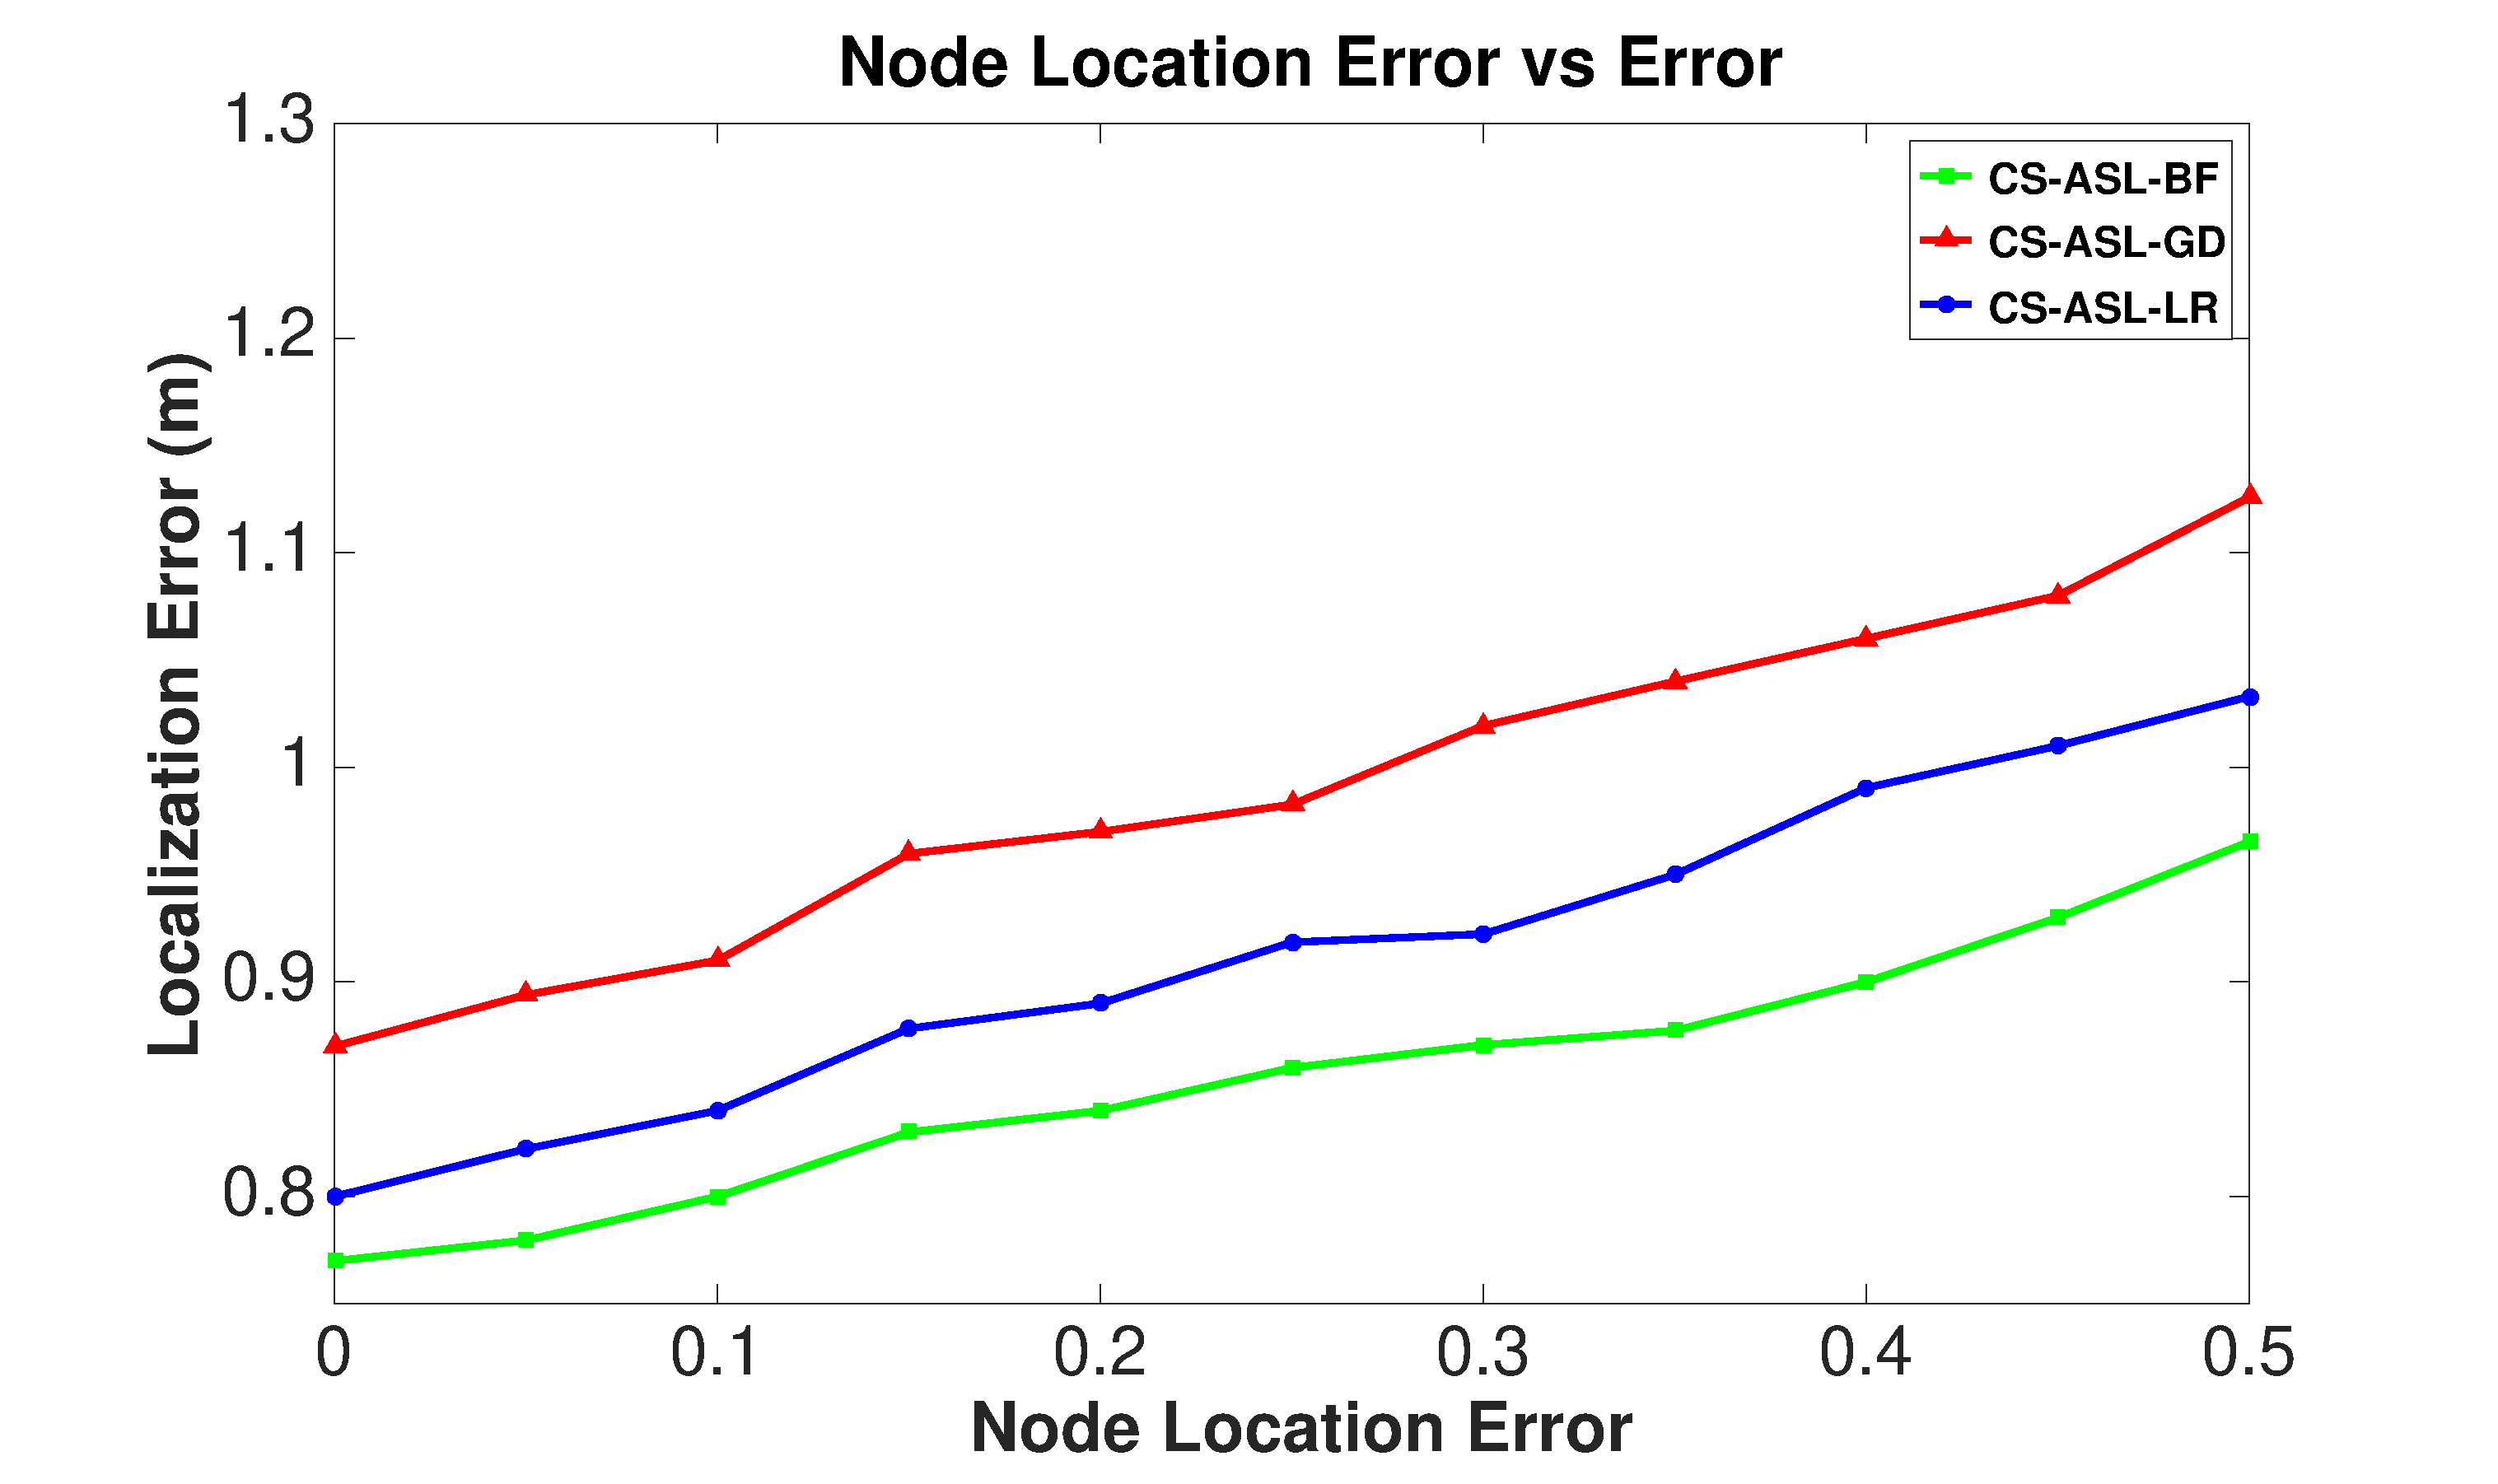
\includegraphics[height=5.0cm,width=7.0cm]{image/locationerror.eps}
            \vspace{25mm}
            \caption{Localization Error vs. Node Location Error}
             \vspace{-5mm}
             \label{fig5}
        \end{figure}
		\fi

\textbf{3) Impact of the node angle error:}
In localization system, node angel is also an essential parameter that influences the property. No matter how the sensor capability improves, the node angle error still exists due to magnetic interference or users' different operations. Here we choose the node angle error from 0 to 10$^{\circ} $ in steps of 1$^{\circ} $, other parameters still the default values.
As is shown in Fig. \ref{Fig3:3-3}, results demonstrate that our methods have a good node angle fault tolerance.

\textbf{4) Impact of bit-flipping number:}
In WASN, bit-flipping severely influences the localization performance. To prove our methods can  refine bit-fllipping, we reversal the 1-bit signals on purpose. In the condition of 30 nodes, we range the bit-flipping number from 0 to 10 in steps of 1, other parameter remain default. Result in Fig. \ref{Fig3:3-4} shows that CS-ASL-BF method performs well when bit-flipping occurs, on the basis of this,  CS-ASL-GD also have a certain ability to refine bit-flipping with the idea of final partly searching.
CS-ASL-LR behaves more approach to CS-ASL-BF method, even the bit-flipping number adds to 10, it can still determine the source location. Therefore, our methods are bit-flipping tolerance.

	\iffalse	
  \begin{figure}[htb]       
           % \centering
			\vspace{-15mm}
            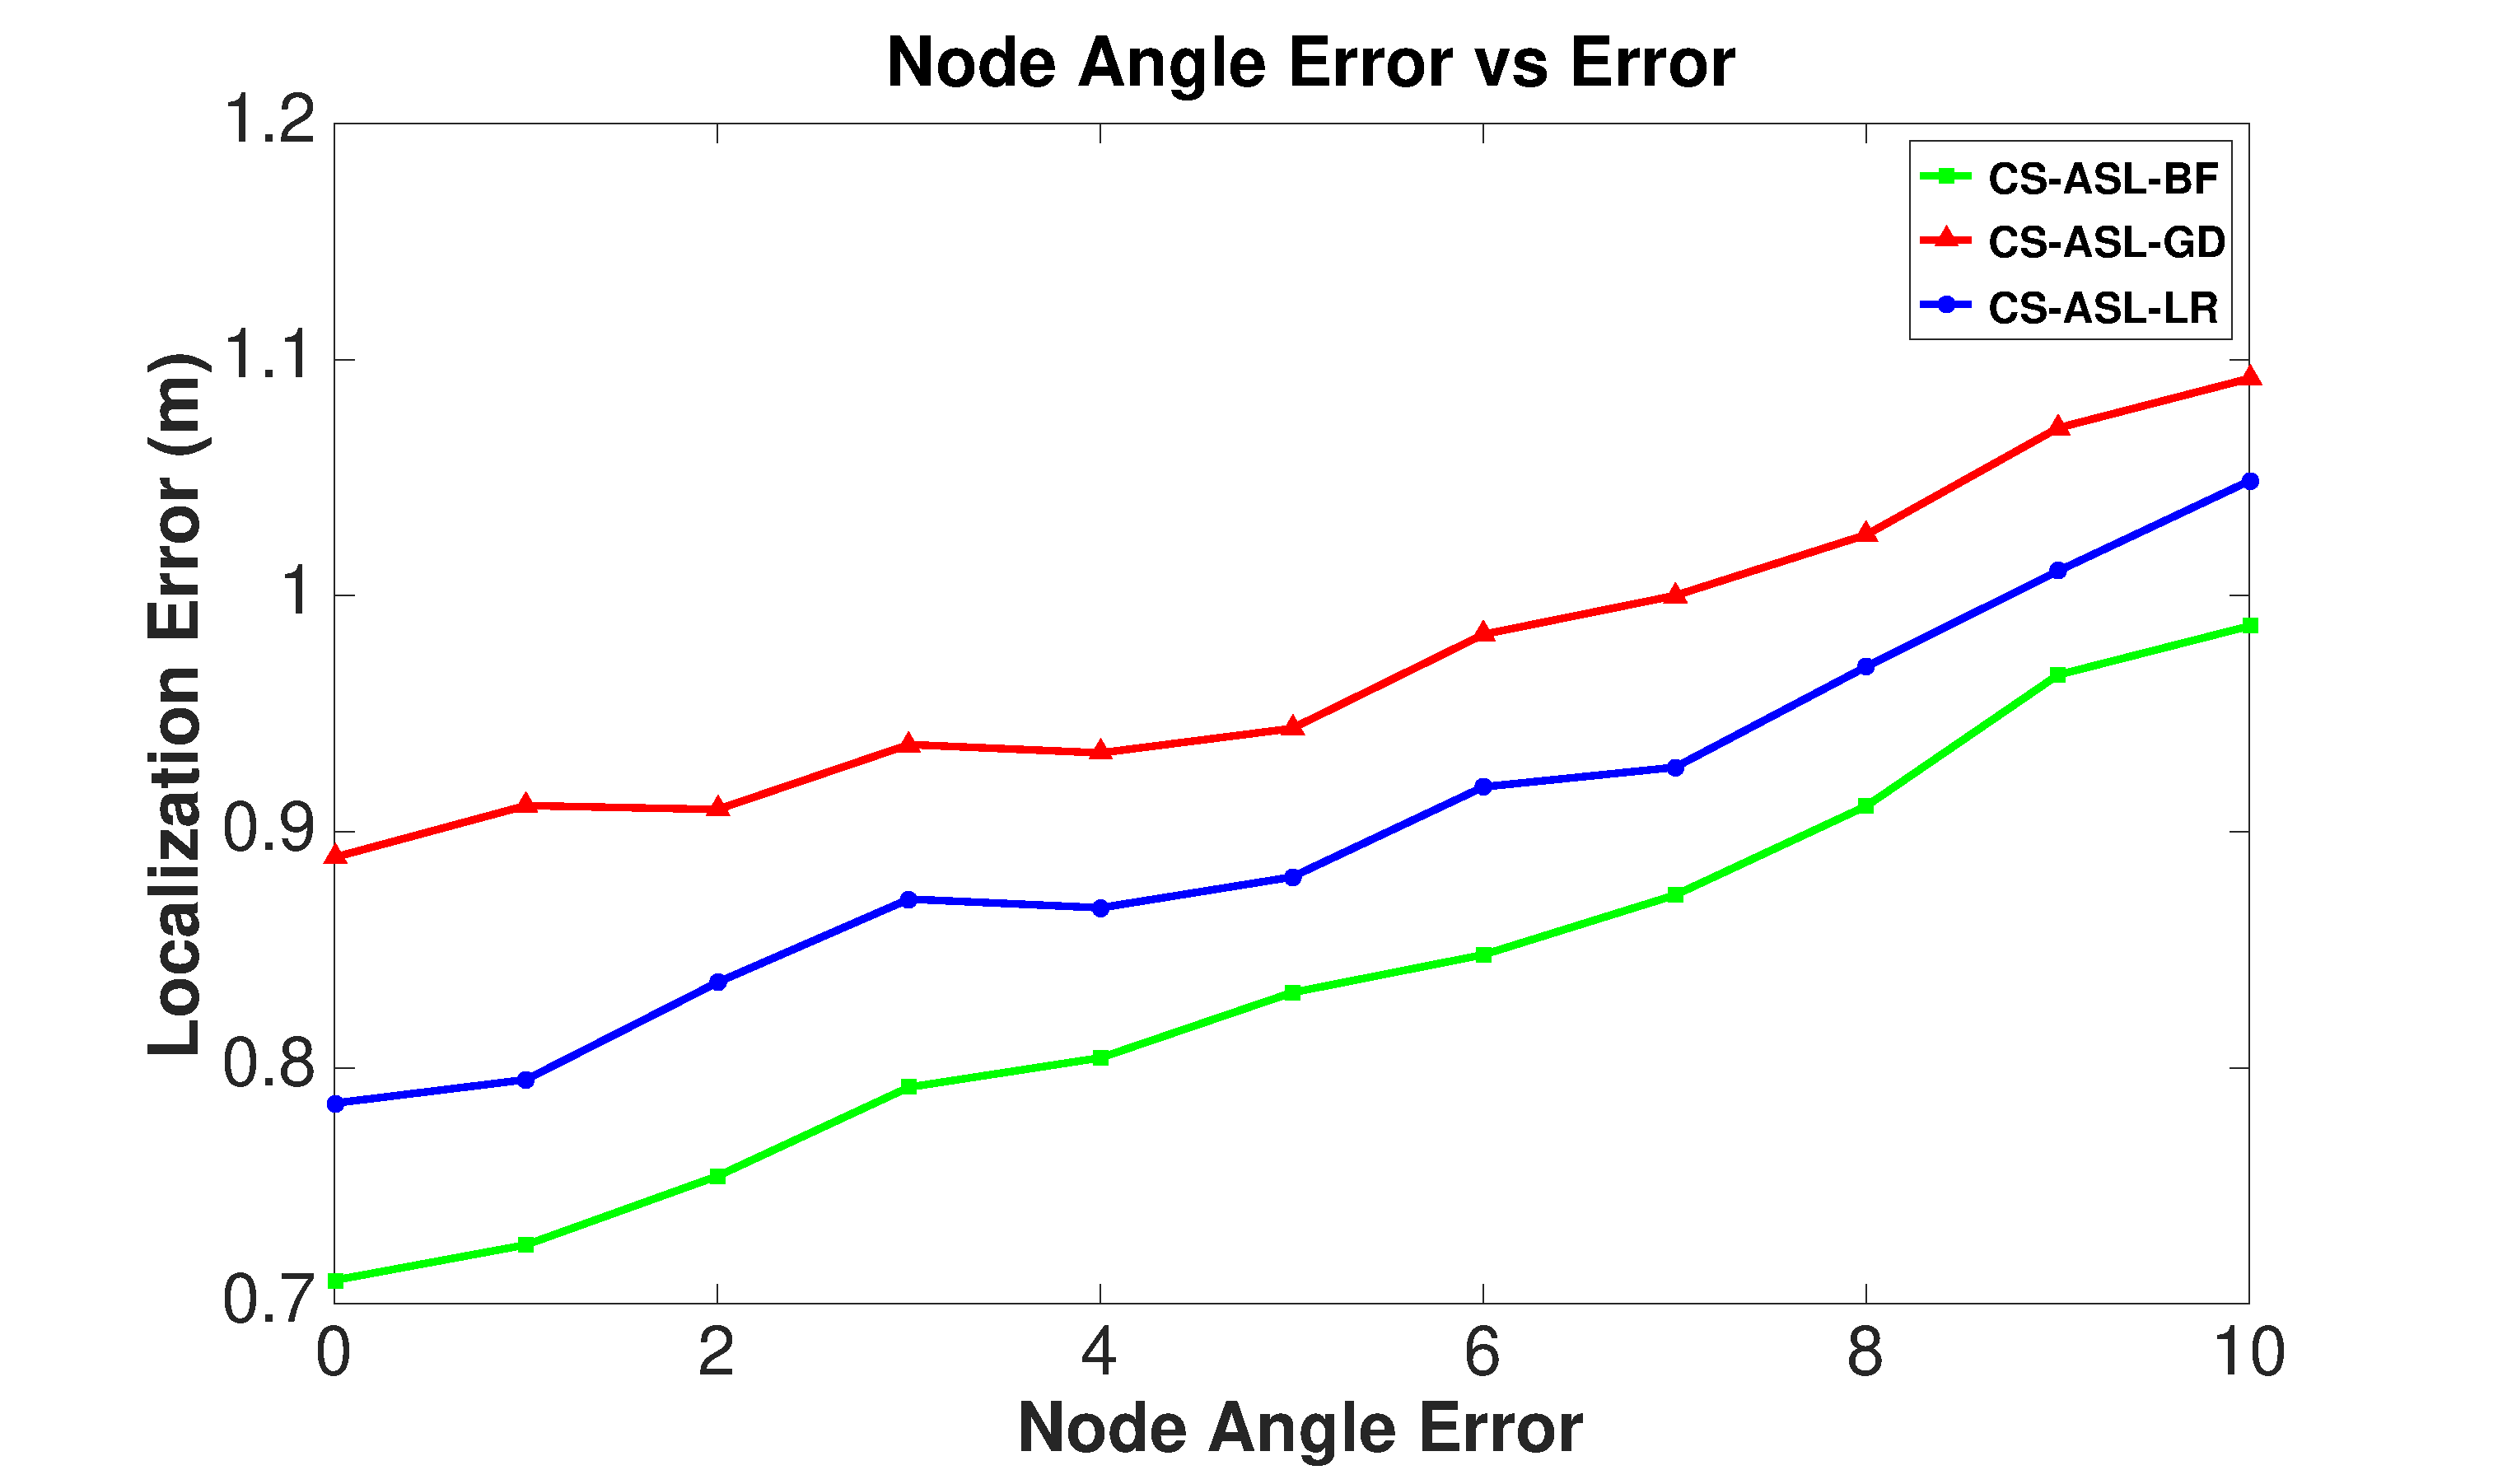
\includegraphics[height=5.0cm,width=7.0cm]{image/angle.eps}
           \vspace{15mm}
            \caption{Localization Error vs. Angle Error}
             \vspace{-5mm}
             \label{fig6}
        \end{figure}

\fi
		

%\subsection{Emulation}


%In this section, we reported system implementation of our design based on smartphone arrays.
%The 30 smartphones are deployed in a size of 16m$\times$10m space and connected by CISCO CVR328W-K9-CN wireless router.
%TPSN protocol is adapted in the proposed HPI-SBL system to realize time synchronization.
%In the experiment, smartphones are randomly deployed in the space, and 100 times localization results are shown in Fig.~\ref{Fig3:3-4}. 
%In the figure, blue squares stand for anchor
%nodes, red circle squares are the real position of acoustic sources and black dots are the estimated location by HPI-SBL. 
%An arrow origins from the estimated location of each acoustic source and points to its real position. 
%As shown in Fig.\ref{Fig3:3-4}, most of estimated locations are close to the ground truth and the errors between them are very small.
%In our experiment, the acoustic sources got localized with average and maximum error of 0.84 feet and 3.91 feet, respectively. Fig.\ref{Fig3:3-4} tells that
%the proposed HPI-SBL successfully accomplishes acoustic source localization with good robustness.

\iffalse
  \begin{figure}[htb]
              %    \centering
			    \vspace{-12mm}
            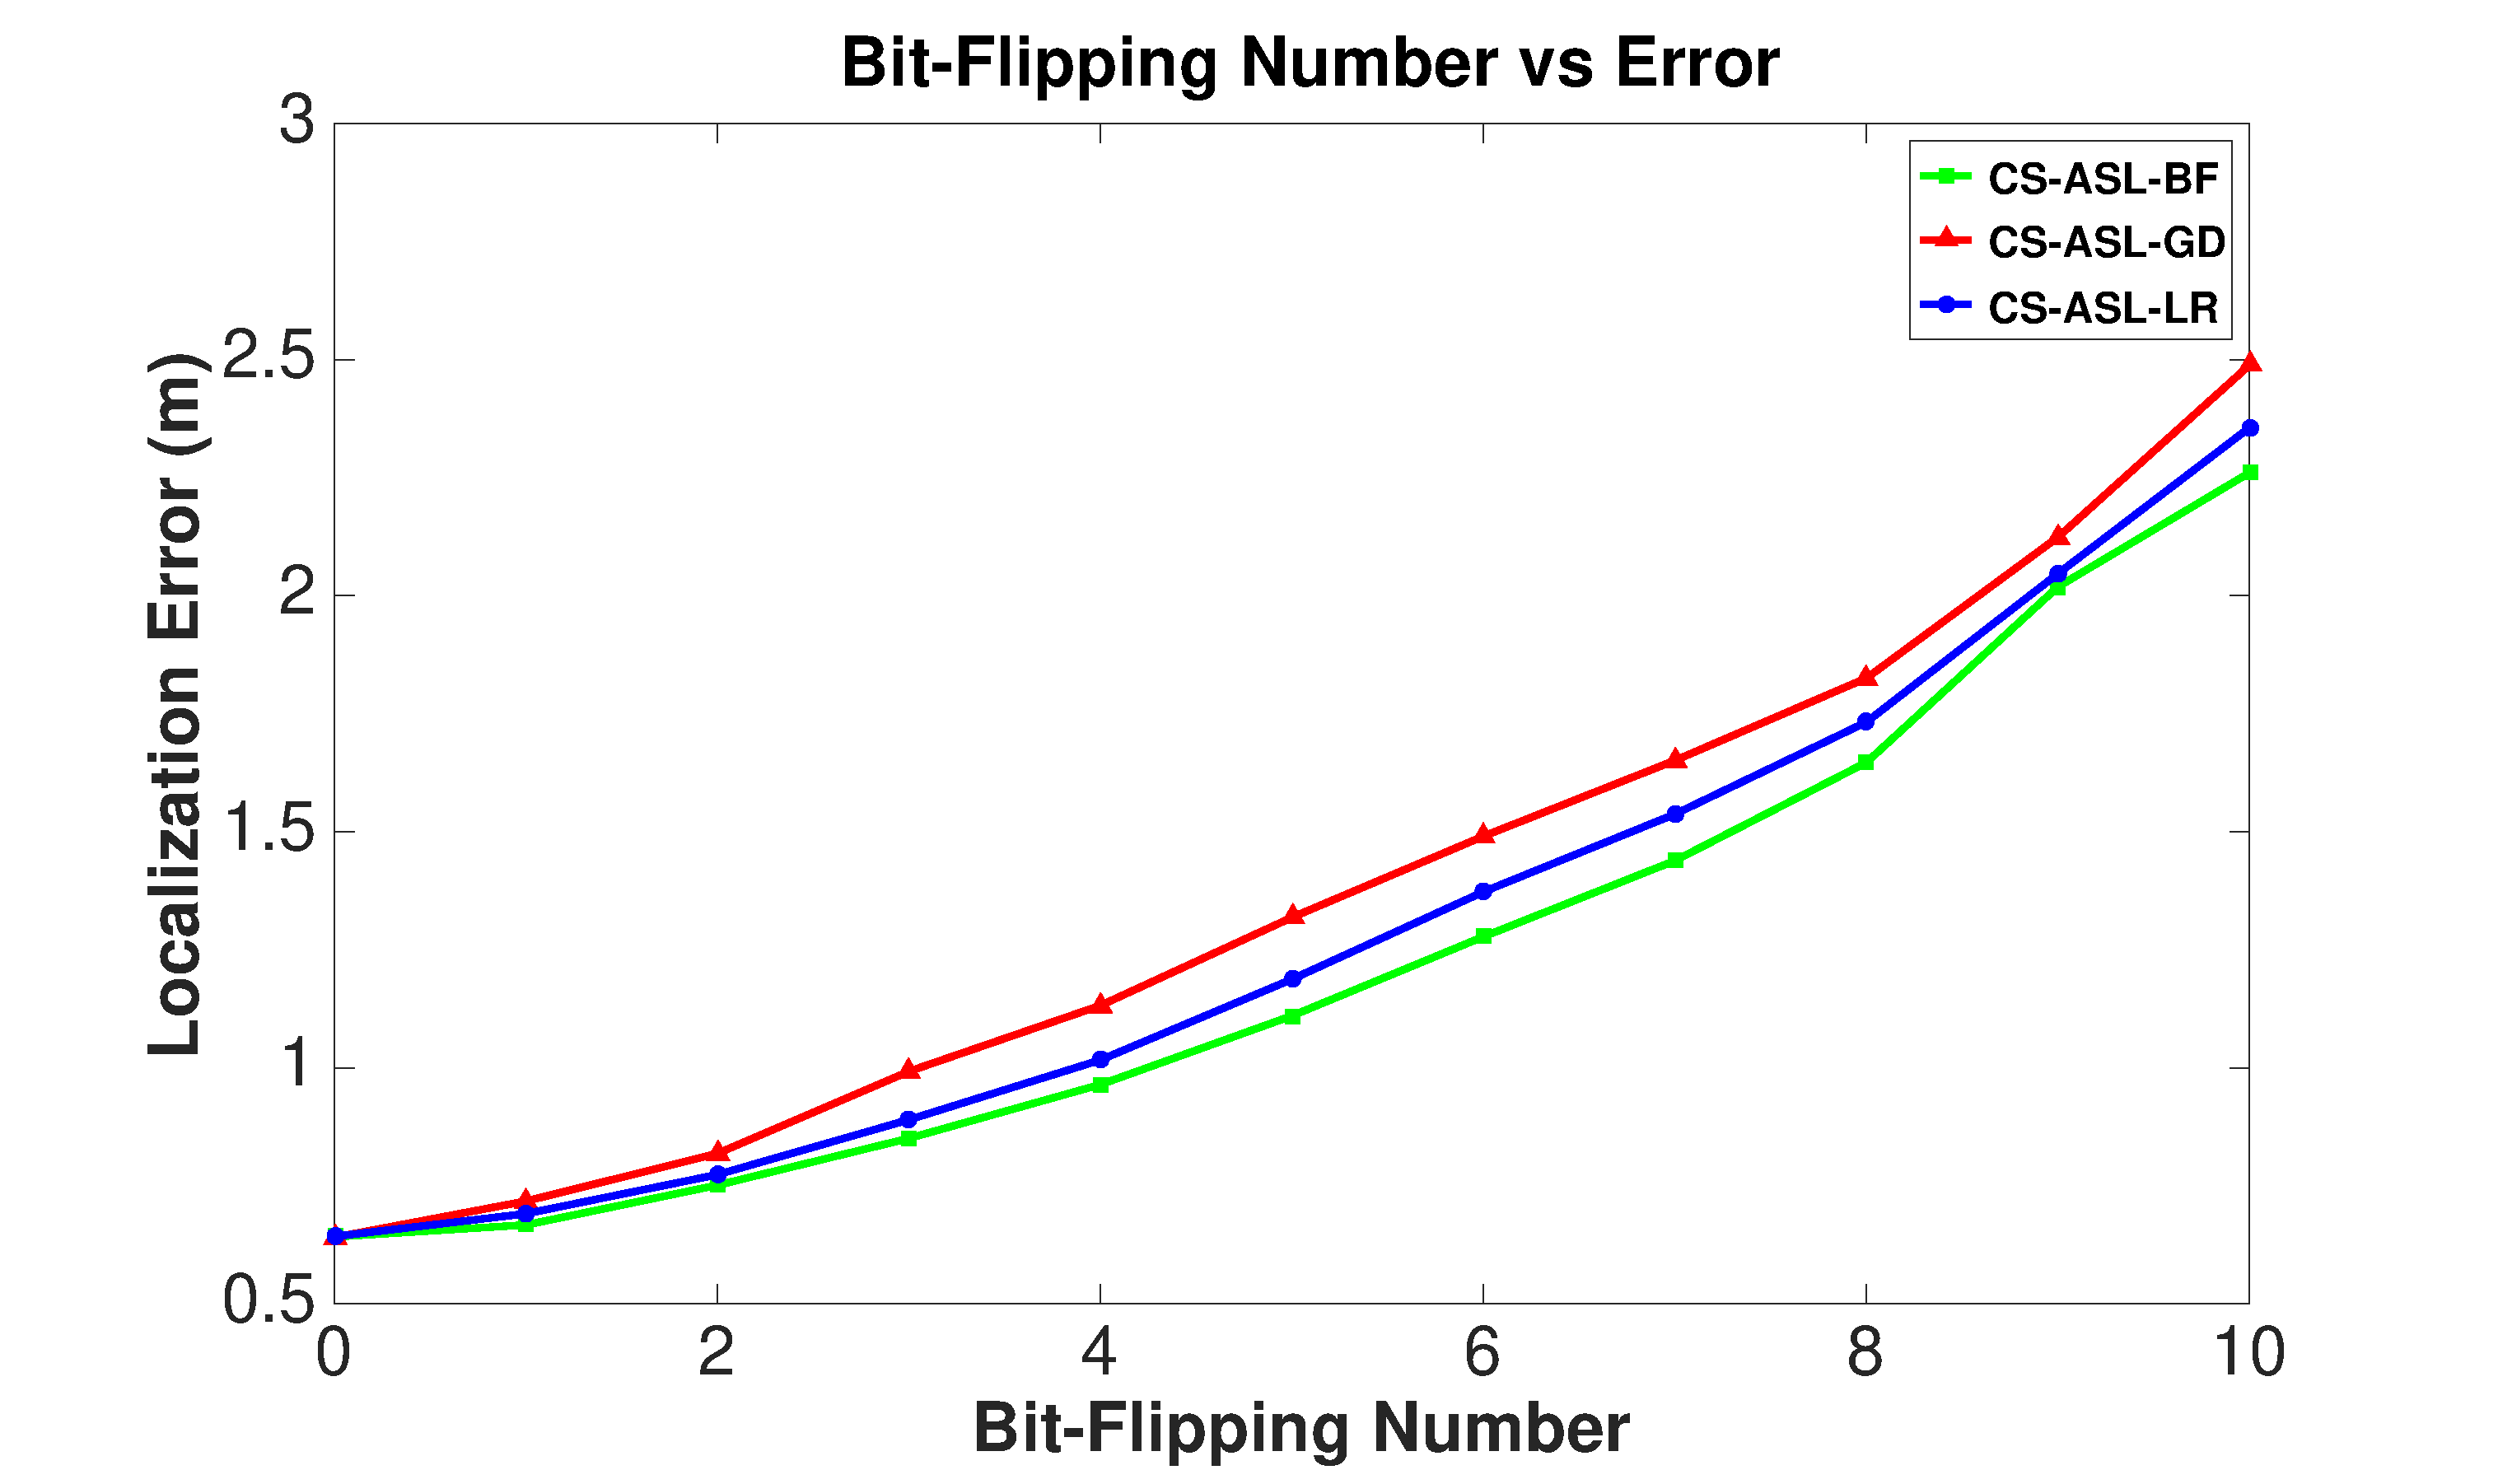
\includegraphics[height=5.0cm,width=7.0cm]{image/errornum.eps}
            \vspace{12mm}
            \caption{Localization Error vs. Error number}
             \vspace{-5mm}
             \label{fig7}
        \end{figure}
\fi
		
		
		
\begin{figure}[hptb]
\begin{center}
\subfigure[Impact of number of anchors]{
\label{Fig3:3-1}
\begin{minipage}[t]{0.46\linewidth}
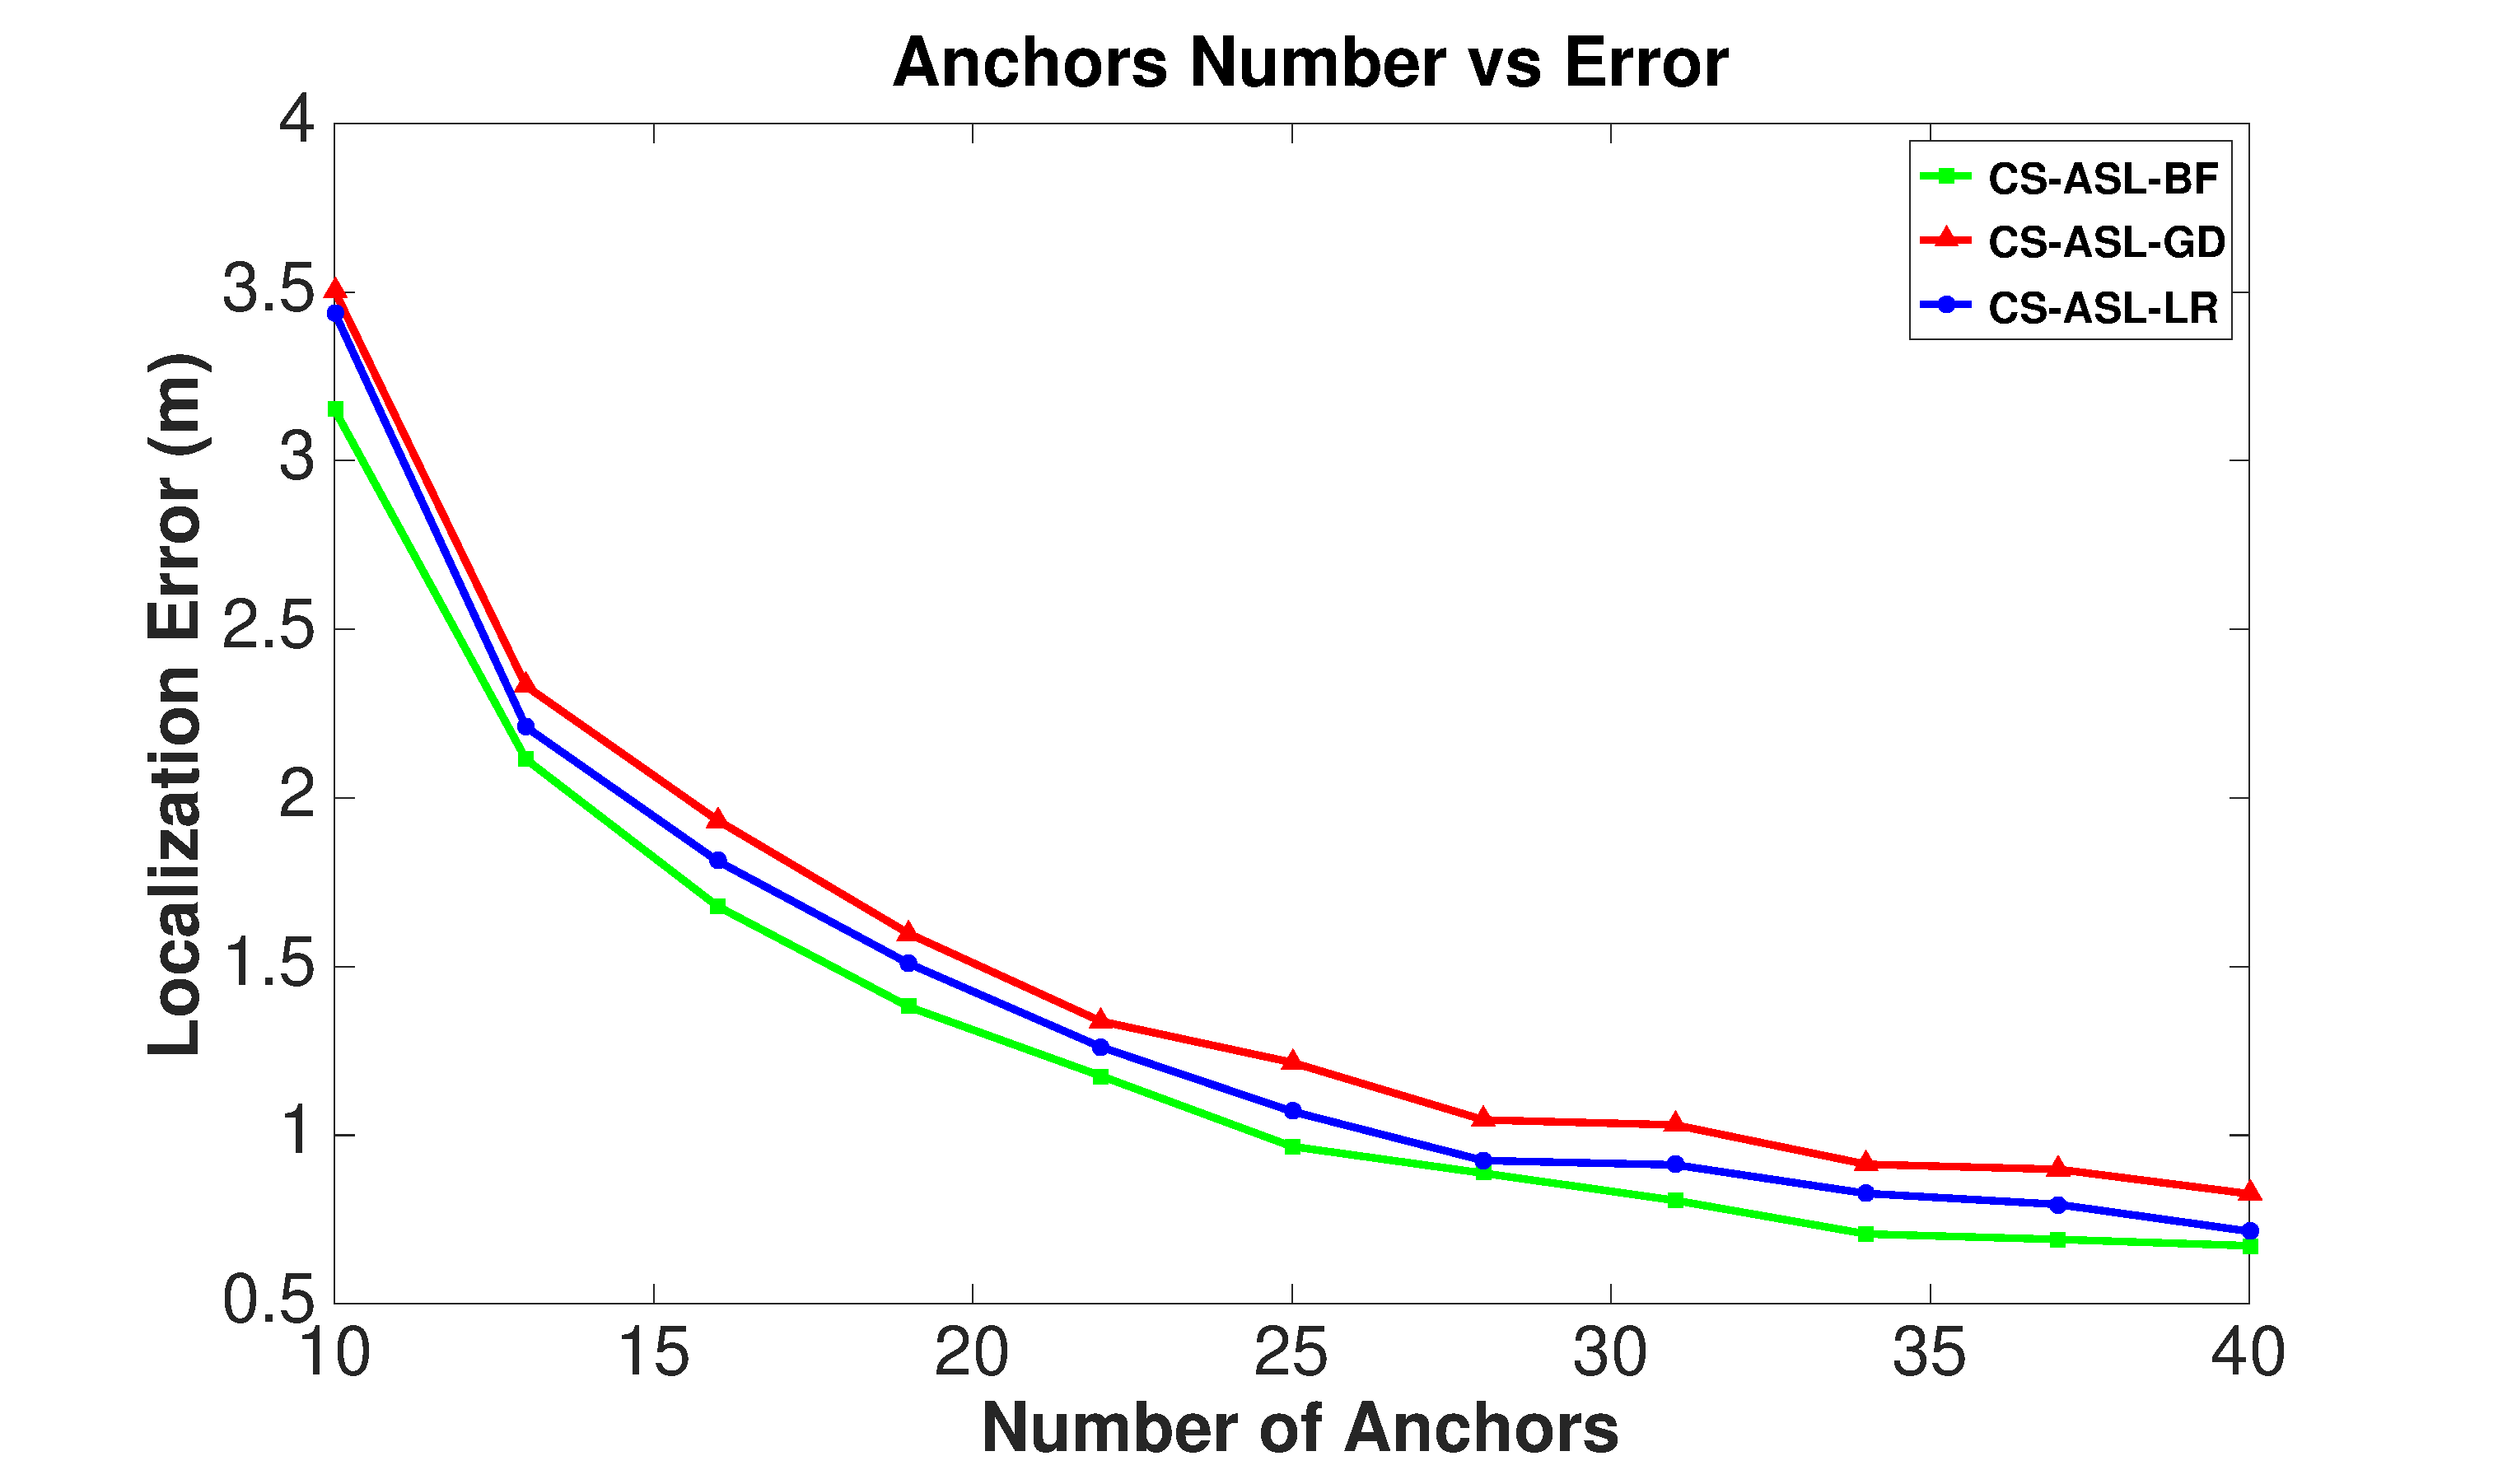
\includegraphics[width=1.150\textwidth]{image/nodenumber.eps}
\end{minipage}
}
\hspace{-0.1in}
\subfigure[Impact of node location error]{
\label{Fig3:3-2}
\begin{minipage}[t]{0.46\linewidth}
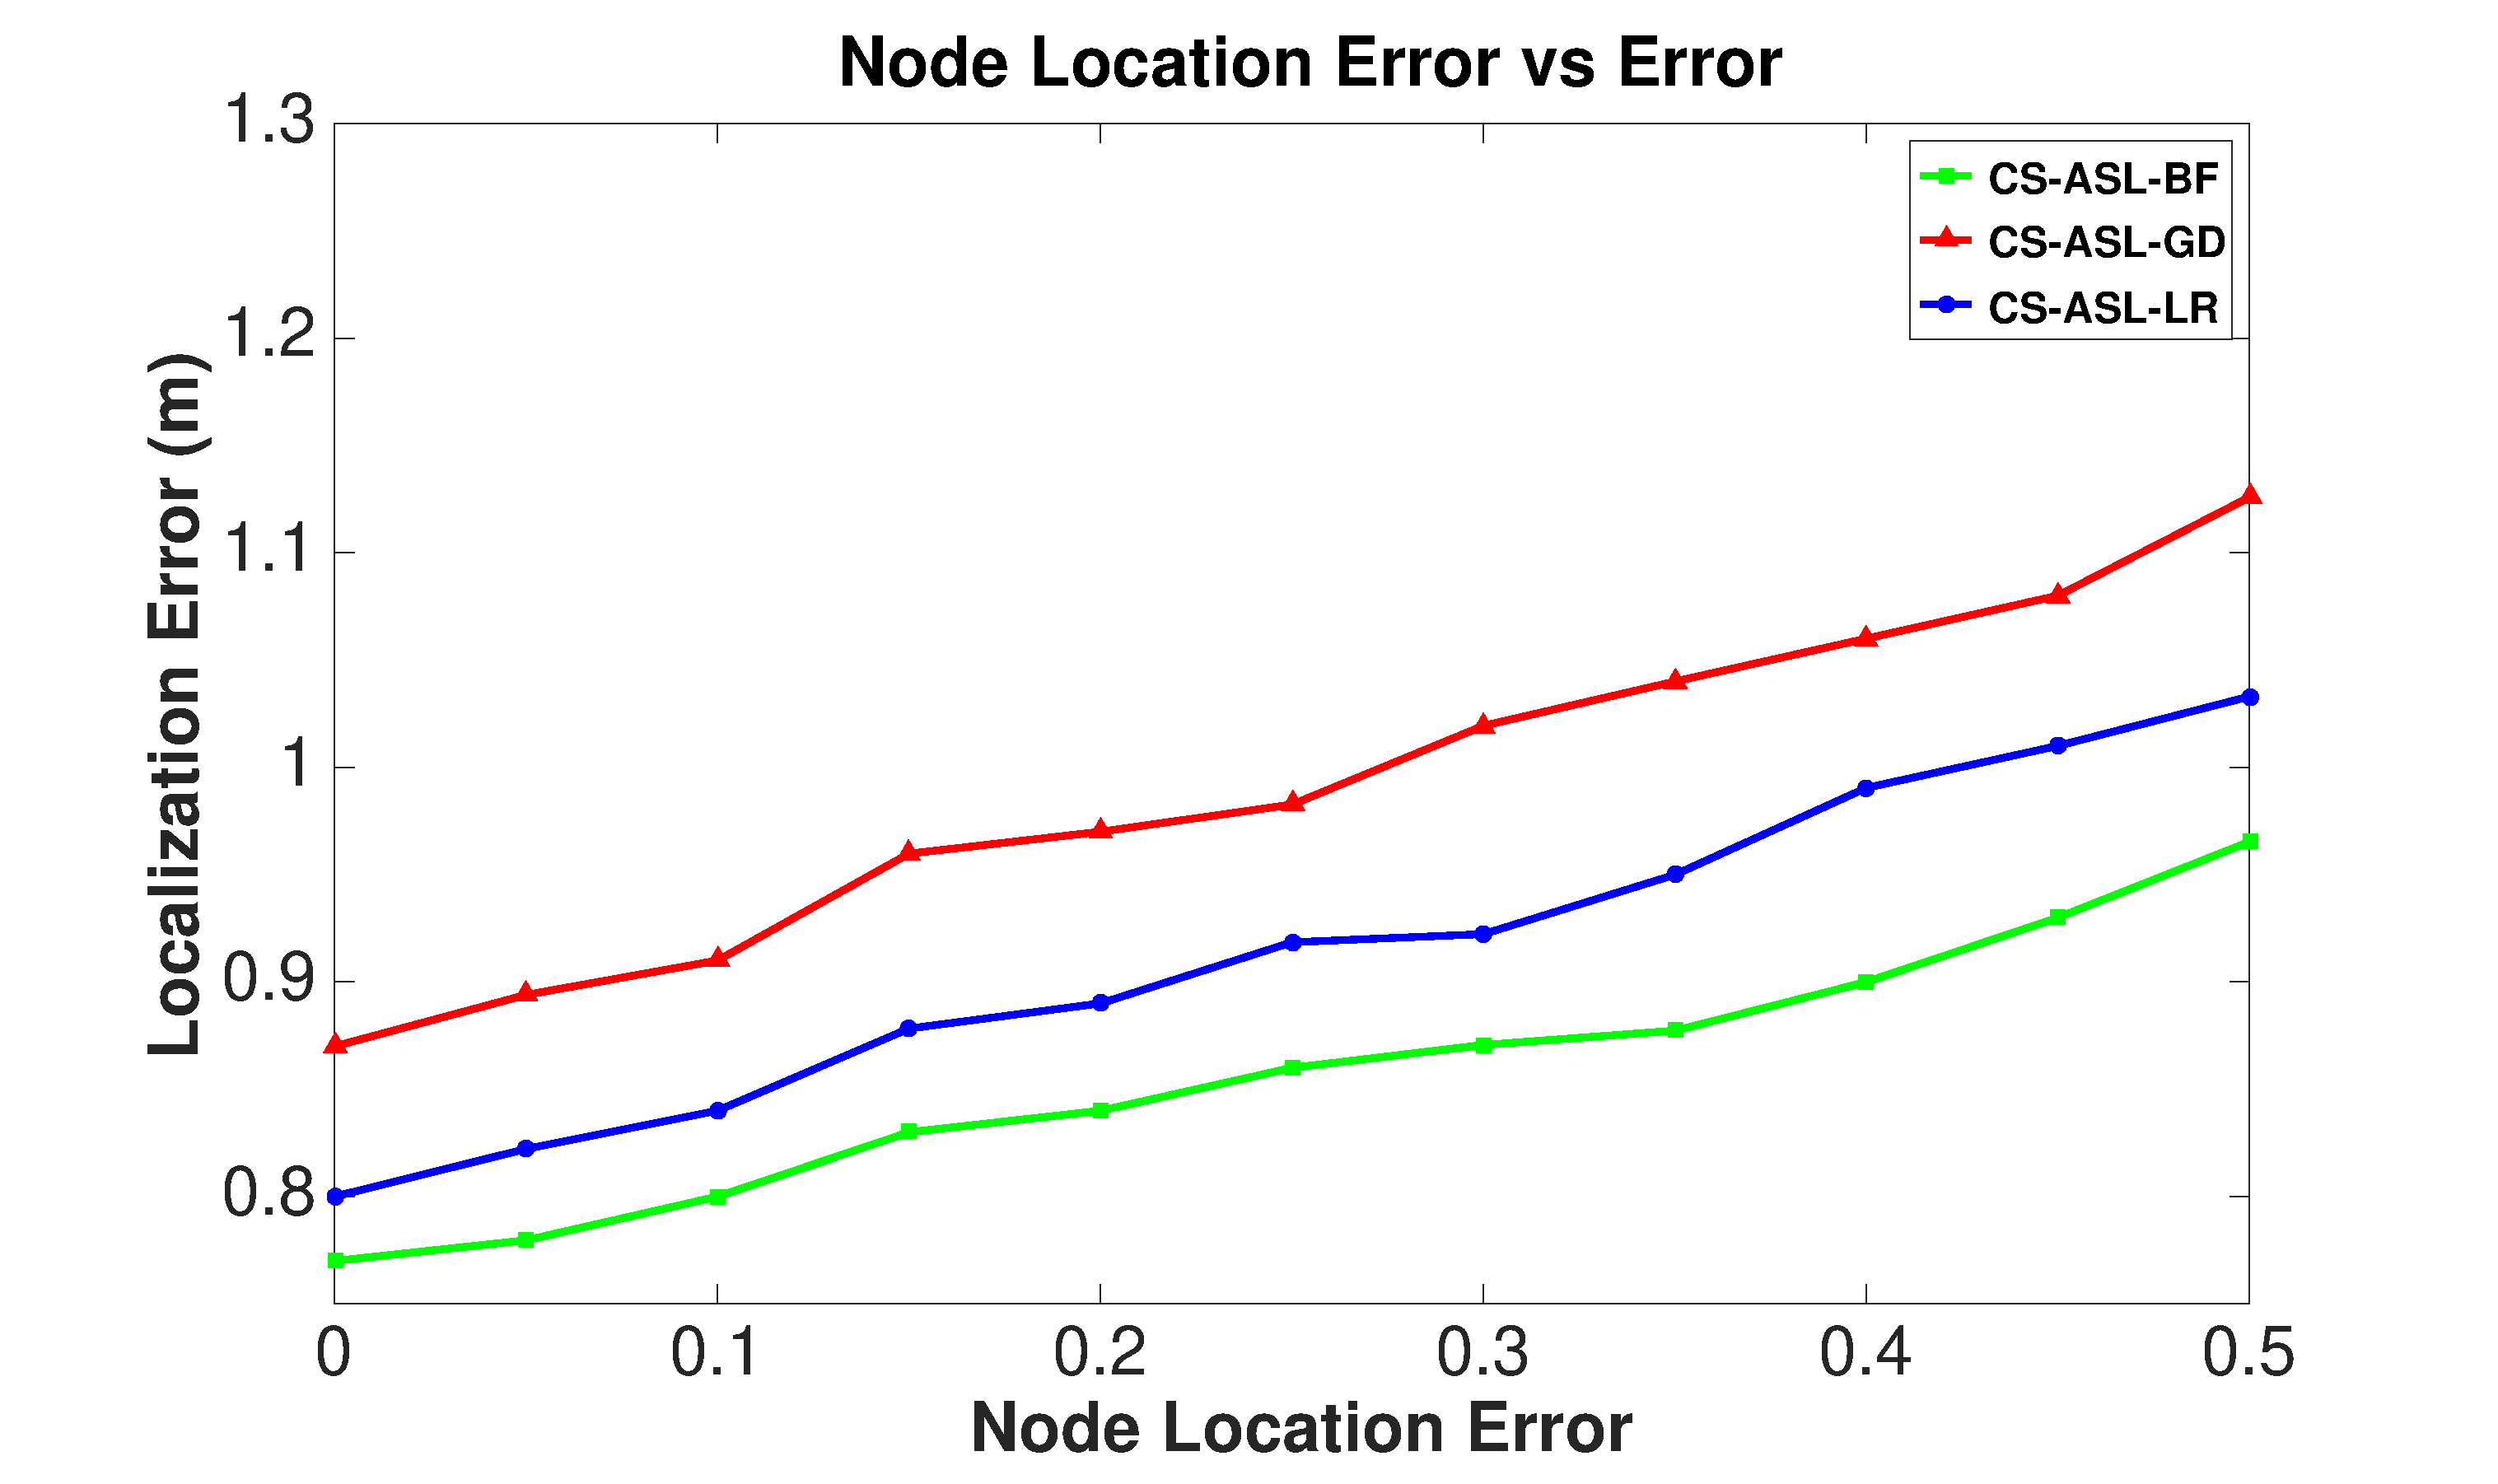
\includegraphics[width=1.150\textwidth]{image/locationerror.eps}
\end{minipage}
}

\subfigure[Impact of angle error]{
\label{Fig3:3-3}
\begin{minipage}[t]{0.46\linewidth}
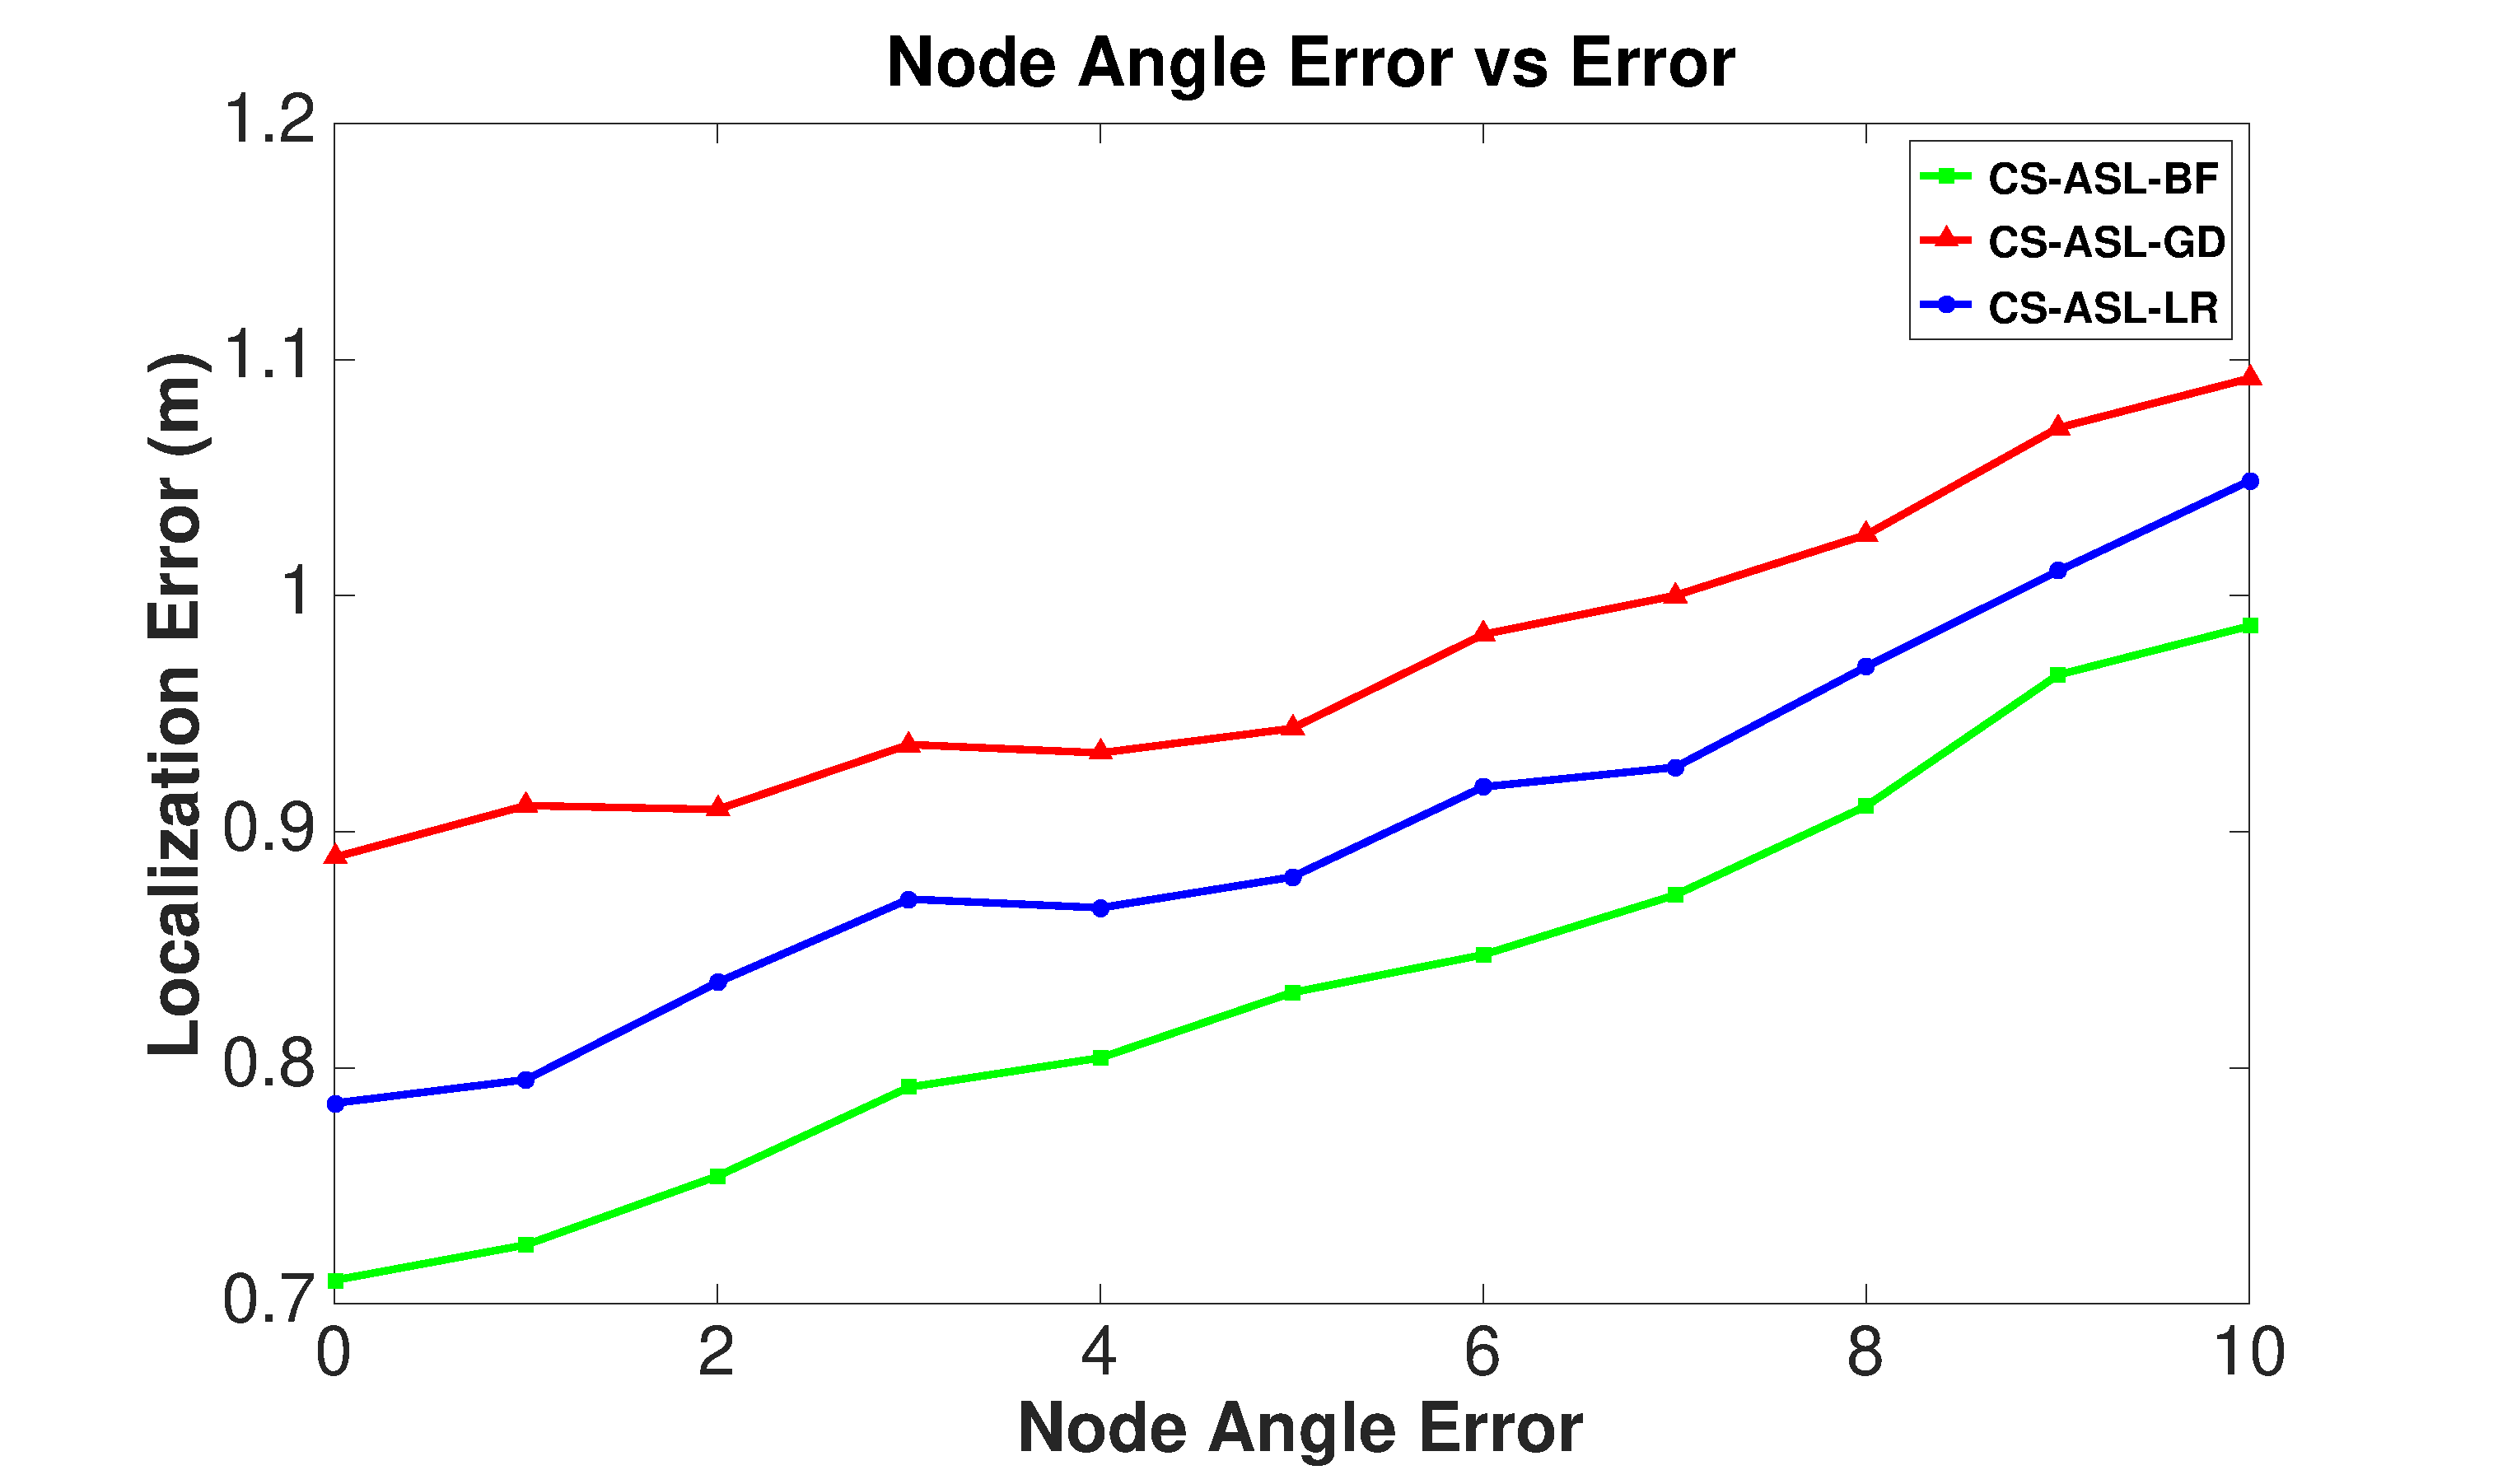
\includegraphics[width=1.150\textwidth]{image/angle.eps}
\end{minipage}
}
\hspace{-0.1in}
\subfigure[Impact of bit-flipping number]{
\label{Fig3:3-4}
\begin{minipage}[t]{0.46\linewidth}
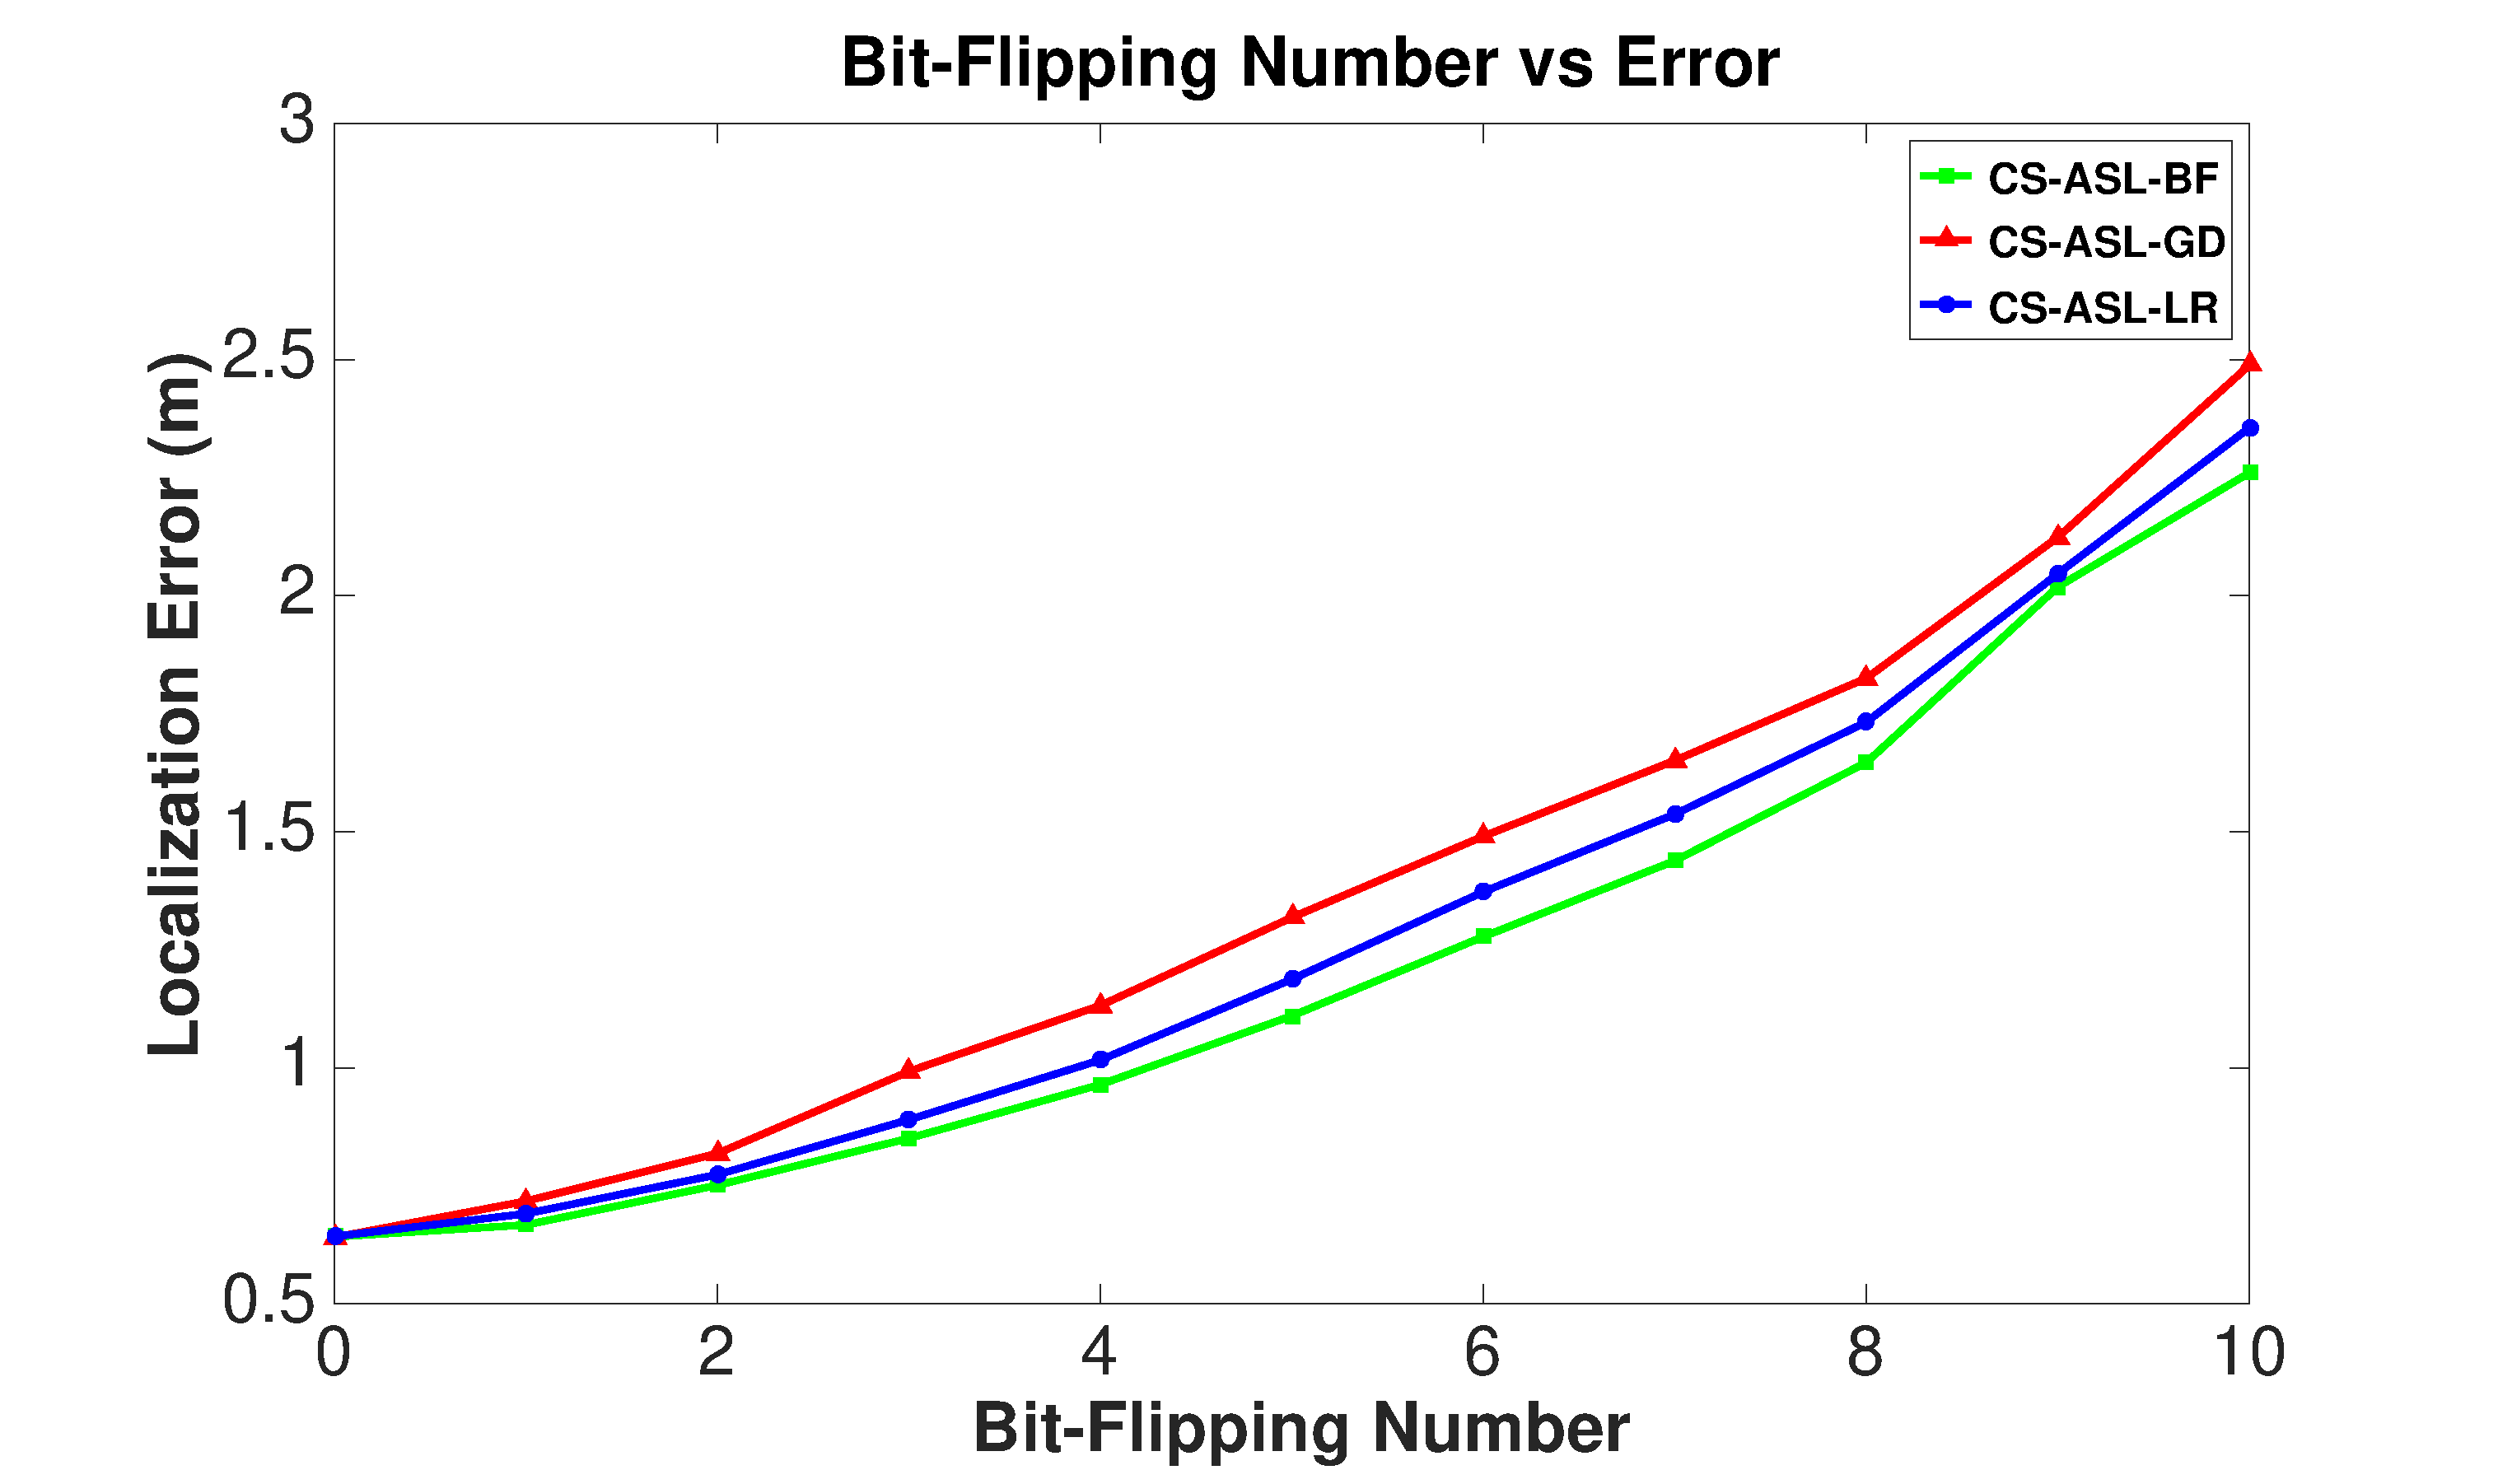
\includegraphics[width=1.150\textwidth]{image/errornum.eps}
\end{minipage}
}
\caption{\label{Fig3:}The results of simulation.}
\end{center}
 \vspace{-5mm}
\end{figure}

\subsection{Testbed Experiment}
In this part, we utilize the testbed experiment to evaluate the performance of our CS-ASL-LR method. We use 30 Redmi smartphones with double microphones as sensors to collect 1-bit datas and connect them through TP-LINK TL-WDR4310 wireless router. We do the experiments for 100 times, every time we deployed the 30 smartphones randomly in an area of 16m$\times$10m, results are demonstrated in Fig.3, blue squares stand for anchor nodes, red circle squares denote the real acoustic sources position and black dots are the estimated location by CS-ASL-LR. An arrow origins from the estimated location of each acoustic source and points to its real position. As shown in Fig.3, most of the estimated locations are close to the ground truth and the errors between them are very small. In our experiment, the acoustic sources got localized with average and maximum error of 0.63 feet and 2.74 feet, respectively. Fig.3 tells that the proposed CS-ASL-LR successfully accomplishes acoustic source localization.

\begin{figure}[htb]
	\centering
	%\setlength{\abovecaptionskip}{-15pt}
	%\setlength{\belowcaptionskip}{-5pt}
	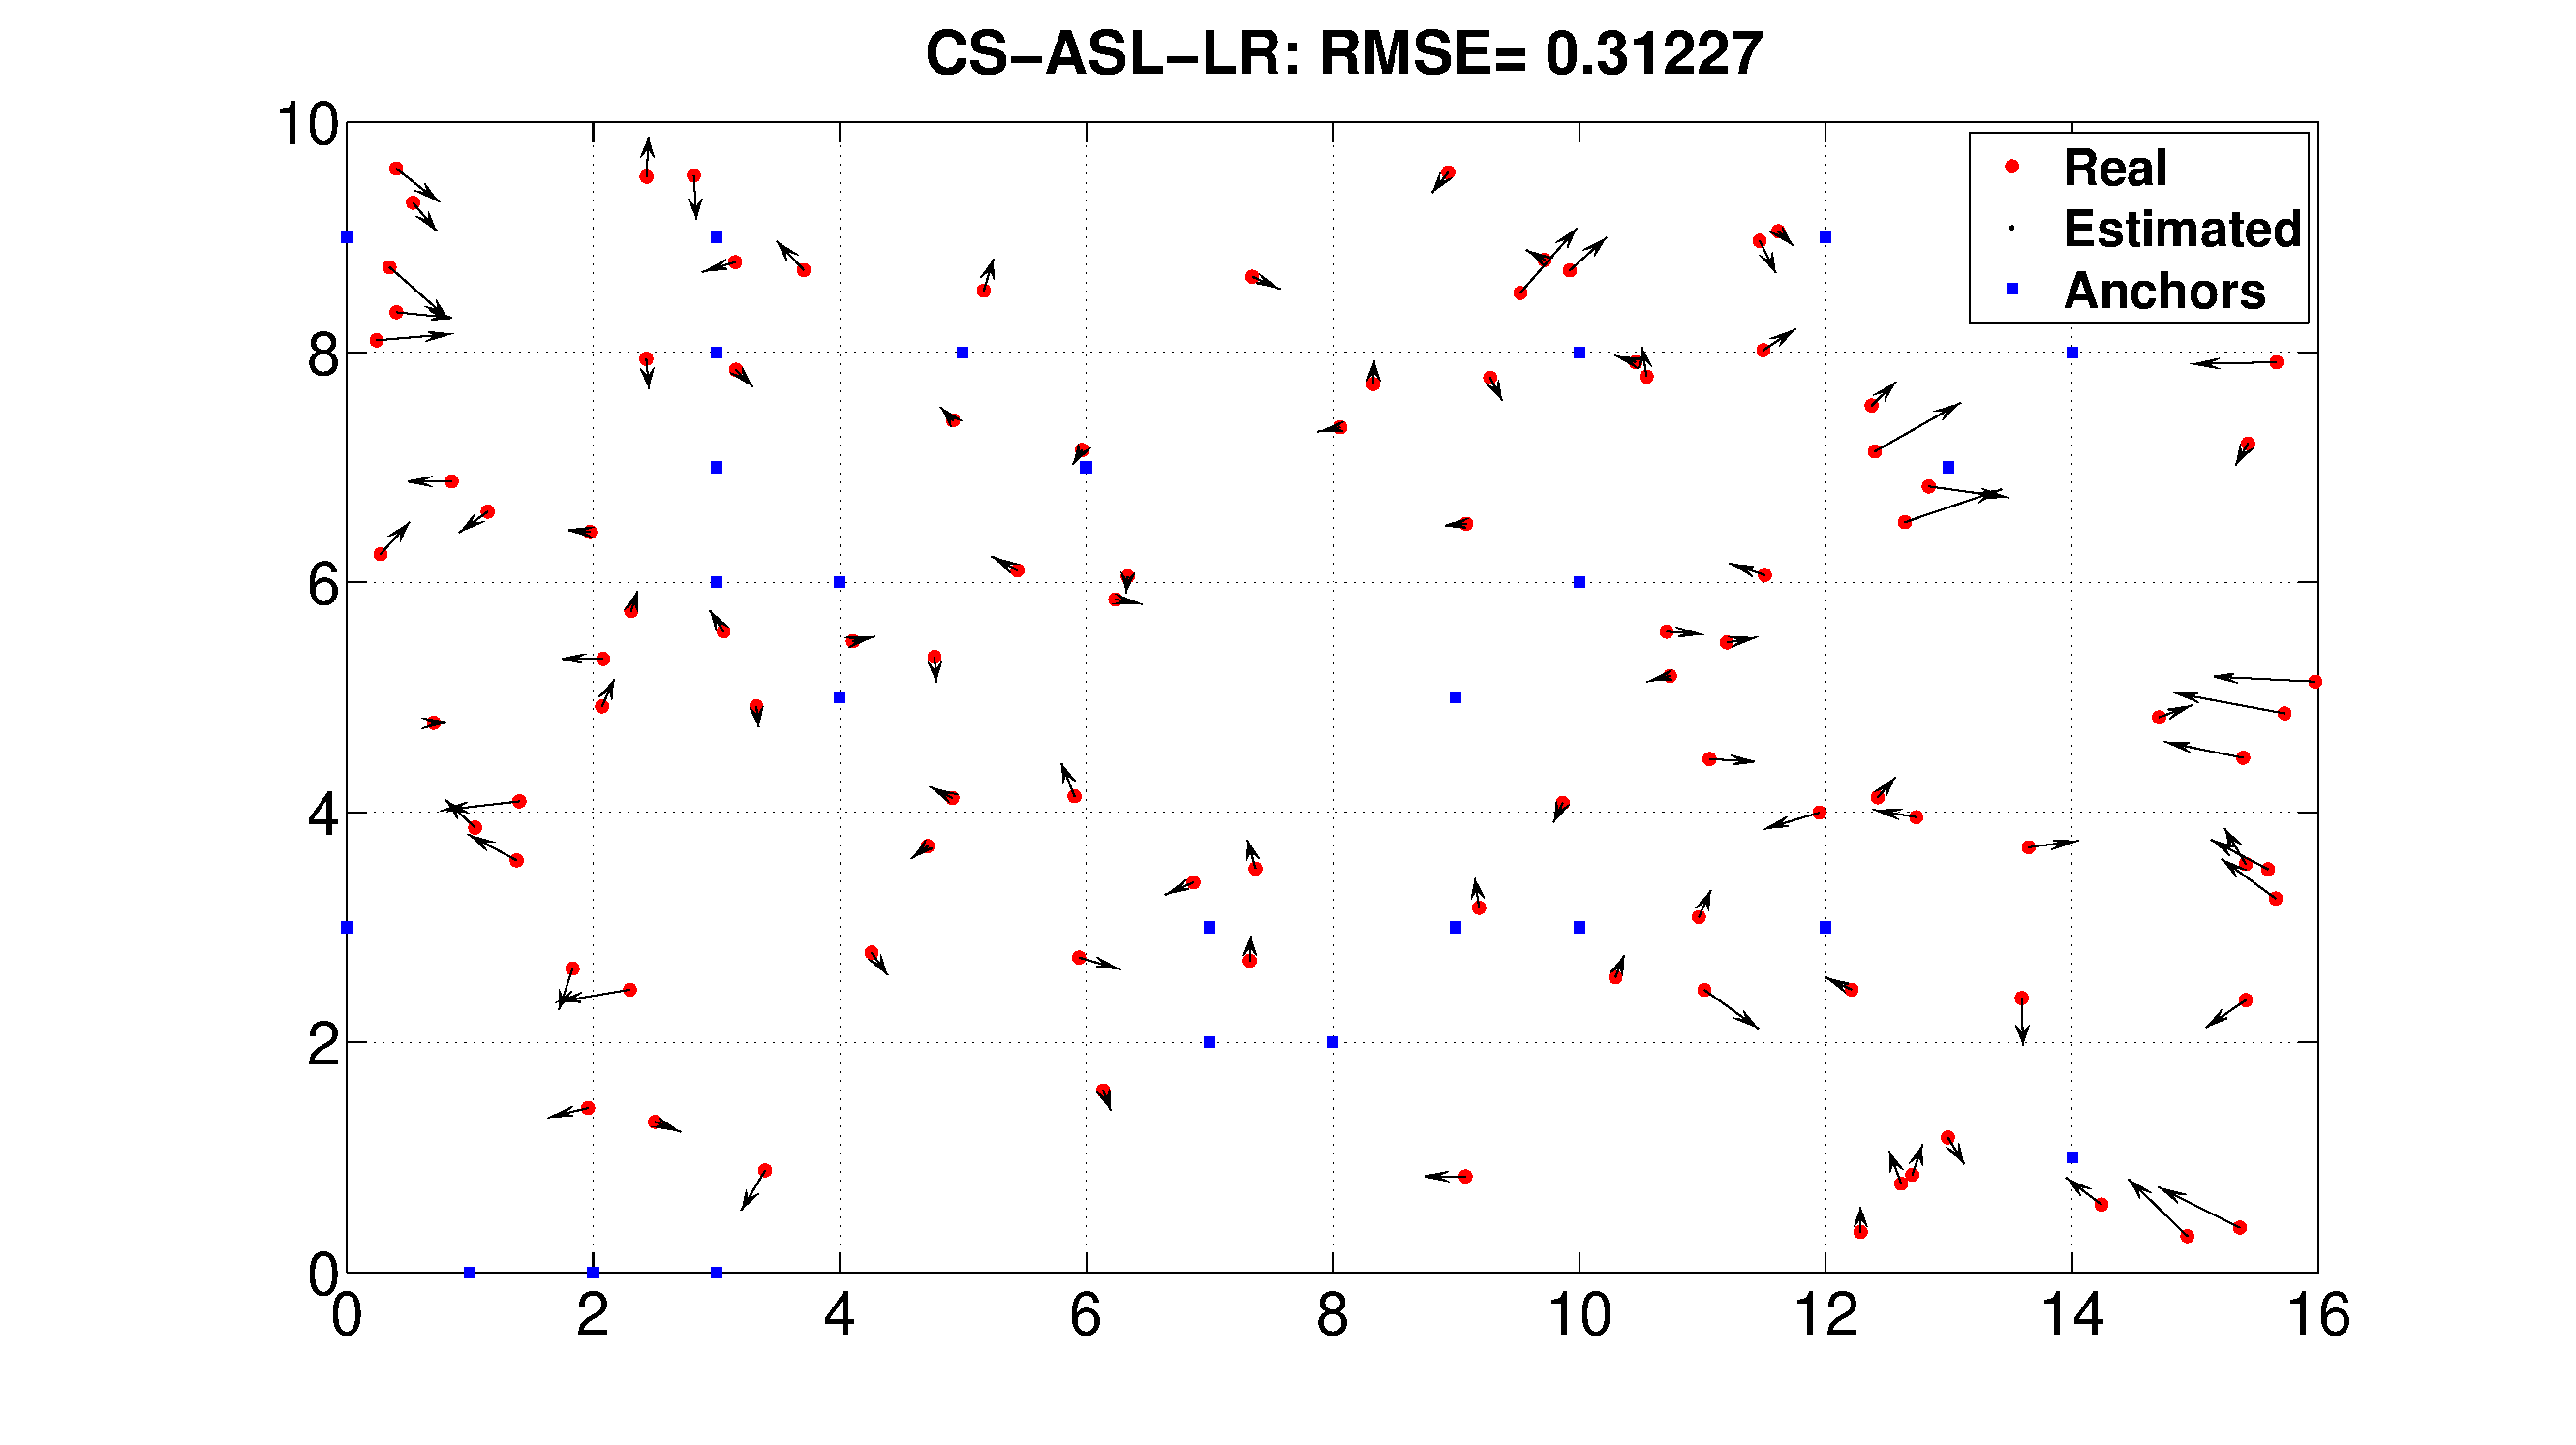
\includegraphics[height=4.5cm]{image/lab.eps} 
	\caption{Testbed experiment}
	\label{overview}
\end{figure} 

 \textbf{Summary:} Considering the parameters including the number of anchors, node location error, angle error and bit-flipping number, simulation results and testbed experiment prove that our methods have a great performance. CS-ASL-BF obtain an accuracy localization result in all fault environment, however, it searches all points every time which slows down the efficiency. CS-ASL-GD based on gradient descent, we make further searching that decrease the final localization error and guarantee the system efficiency even with bit-flipping. CS-ASL-LR takes more step to improve the localization accuracy. Above all, our methods can accomplish localization with robustness.
%%%%%%%%%%%%%%%%%%%%%%%%%%%%%%%%%%%%%%%%%%%%%%%%%


%\section{Related Work}

Acoustic source localization in sensor network is a widely-studied problem. 
In the past few years, there has been a growing interest for spatial distributions of independent (unsynchronized) acoustic sensors, each made of two or more synchronized microphones. Due to space constraints, we can only mention a few directly related works here.
% Omologo, \emph{et al.} \cite{omologo1994acoustic} compute the Steered Response Power maps associated to all the microphone pairs over a spatial grid and then localize the source
% as the peak of the cumulative global map, with overall computational costs that are often too demanding for the application at hand.
% Better computational efficiency is achieved in \cite{cobos2011modified} where the SRP  accommodates a different computation over a coarser grid.
% Alternate approaches based on Least Squares were proposed in \cite{rabinkin1996dsp} with a certain sensitivity to environmental noise;
% and in \cite{do2007real} where a stochastic region contraction of the grid was proposed, adopting a multi-resolution approach.
Wang, \emph{et al.} \cite{wang2003acoustic} described a system having static cluster architecture, the system experienced a problem in that the accuracy decreased when an acoustic source occurred between the clusters.
Chen, \emph{et al.} \cite{chen2004dynamic} showed that nodes in the system did not need to recognize their cluster head, reducing the constraints on deployment of the localization system.
Hu, \emph{et al.} \cite{hu2009design} design the system based on 2-tier architecture, which experienced cost and deployment problems especially in the very large target area.
Rabbat, \emph{et al.} \cite{rabbat2005robust} proposed a decentralized algorithm based on the distributed ML estimation technique using token ring architecture.
Kim, \emph{et al.} \cite{kim2009locating}proposed to identify the node closest to the acoustic source, based on TOA comparisons between all nodes, thus incurring high communication cost and requiring global synchronization between all sensor nodes.
Lightning is a method proposed in \cite{wang2008lightning} to identify the sensor closest to the acoustic source, also based on expensive broadcasting/flooding.
Aarabi, \emph{et al.} ~\cite{aarabi1900fusion} used 10 dual-microphone arrays distributed in a room and used their data to locate three speakers.
Wu, \emph{et al.} ~\cite{wu2012fusion} used three dual-microphone arrays to locate two sound sources in a distributed way in which only the local DOA estimates are communicated among arrays.
Canclini, \emph{et al.}\cite{canclini2013acoustic,Canclini2015} proposed a method for localizing an acoustic source with distributed microphone networks based on TDOA between microphones of the same sensor.

Most of the existing acoustic source localization methods in sensor networks are based on range-based measurement.
In contrast, our work is a range-free method and shown to be robust to the errors of node locations and the errors of measurements.
There have existed some research on range-free localization method.
Yedavalli, \emph{et al.} ~\cite{yedavalli2008sequence} proposed a Sequence-Based Localization(SBL) in WSN. 
The heart of SBL is the division of a 2D localization space into distinct regions by the perpendicular bisectors of lines joining pairs of reference nodes (nodes with known locations).
%Each distinct region formed in this manner can be uniquely identified by a location sequence that represents the distance ranks of reference nodes to that region. 
%The unknown node first determines its own location sequence based on the measurement between itself and the reference nodes, then searches through the location sequence table to determine its location.
In their earlier work \cite{yedavalli2005ecolocation}, Ecolocation used location constraints for robust localization.
%A location constraint is a relationship between the distances of two reference nodes from the unknown node that determines its proximity to either
%reference nodes. Location constraints can be graphically represented by perpendicular bisectors
%between reference nodes, and each location sequence can be written as a set of location constraints.
%Thus, the location constraint set is also unique to each region in the arrangement.
Chakrabarty, \emph{et al.} \cite{chakrabarty2002grid} and Ray, \emph{et al.} \cite{ray2004robust} use identity codes to determine the location of sensor nodes in grid and nongrid sensor fields, respectively. 
% Here, each grid point or region in the localization space is identified by a unique set of reference node IDs whose signals can reach
% the point or region, and this unique set is an identity code for that point or region. 
% The two main drawbacks of this
% approach are that 1) in order to uniquely identify all unknown node locations in the localization space, the reference nodes need to be placed carefully according to
% rules determined by an optimization algorithm, and that 2) for acceptable location accuracies, the number of reference nodes required is prohibitively expensive, and for
% sparse networks of reference nodes, the accuracy is coarse grained in the order of radio range. 
He, \emph{et al.} \cite{he2003range} propose an RF-based localization technique in which the unknown node location is determined by the intersection of all triangles,
formed by reference nodes, that are likely to bound it. The unknown node determines its existence inside a triangle by
comparing its measured RSS values to that of its neighbors to detect a trend in RSS values in any particular direction
This technique depends on the weak assumption that signal strength decreases monotonically with distance, which is not true in real-world scenarios.
Zhong, \emph{et al.} \cite{zhong2009tracking} convert the original tracking problem to the problem of finding the shortest path in a graph, which is equivalent to optimal matching of a series of node sequences. 
Zhong, \emph{et al.} \cite{zhong2009achieving} introduce a proximity metric called RSD to capture the distance relationships
among 1-hop neighboring nodes in a range-free manner. With little overhead, RSD can be conveniently applied as a transparent
supporting layer for state-of-the-art connectivity-based localization solutions to achieve better accuracy.






\section{Conclusions}


In this paper, we have designed and implemented CS-ASL, which leverages dual-microphone smartphone array to achieve acoustic source localization using unreliable binary node sequences.
%
The proposed design formulates acoustic source localization as the sparse recovery problem of 1-bit compressive sensing  by making use of the binary sequence from the smartphone array. Since our system runs on COTS smartphones and supports spontaneous setup, it has potential to enable a wide range of distributed acoustic sensing. Besides the CS-ASL-BF, CS-ASL-GD and CS-ASL-LR are proposed for further enhancing system robustness.
%
Our methods are verified and evaluated through analysis and experiments. According to the results, our method can effectively implement robust acoustic source localization with light communication overhead. 
%
%Our next step is that designing the scheme to find the smartphones with bit-flipping in the sensor network to further improve the performance of the localization system.


% \section{Acknowledge}

% This work is supported by Natural Science Foundation of China (Grants No. 61272524 and No.61202443) and the Fundamental Research Funds for the Central Universities (Grants No.DUT15QY05 and No.DUT15QY51). 
% This work is also supported by Specialized Research Fund for the Doctoral Program of Higher Education (Grant No. 20120041120049).



\bibliographystyle{IEEEtran}
\bibliography{Main}

\end{document}
